\documentclass[a4paper,11pt]{article}
\usepackage[T1]{fontenc}		% Seleção de códigos de fonte
\usepackage[utf8]{inputenc}		% Codificação do documento (conversão
\usepackage{indentfirst}		% Indenta o primeiro parágrafo de cada seção.
\usepackage{graphicx}			% Inclusão de gráficos
\usepackage{subcaption}				% enables the use of subfigures in floats
\usepackage[
%	a4paper,
left=2cm,
right=1.5cm,
bottom=1.5cm,
top = 2.5cm, 
foot=0.7cm]{geometry}
\usepackage{url}
\usepackage{setspace}
\usepackage{amsmath}
\usepackage{amsfonts}
\usepackage{fancyhdr}
\usepackage{multirow}
\usepackage{tabularx}
\usepackage{placeins}
\usepackage{natbib}
\usepackage{import}
\usepackage[nottoc]{tocbibind} % insere as referências no sumário
\usepackage[brazil]{babel}
\usepackage{hyperref}
\usepackage{float}

\pagestyle{fancy}
\fancyhf{}
\lhead{EEL5193 - Máquinas e Acionamentos Elétricos para Automação}
\rhead{Trabalho 2}
\rfoot{\thepage}

\begin{document}
	\thispagestyle{empty}
\begin{center}
	
\includegraphics[height=2cm]{imagens/logoUFSCsimples.png} \\
	{\Large Universidade Federal de Santa Catarina -- UFSC} \\
	{\Large Centro Tecnológico -- CTC} \\
	{\Large Departamento de Automação e Sistemas -- DAS} \\
	\vspace{1cm}
	{\large Disciplina EEL5193 - Máquinas e Acionamentos Elétricos para Automação} \\
	\vfill
	\large{\textbf{Máquinas Elétricas} \\
	} 
	\vspace{1cm}
	% Integrantes: \\
    Bruno Machado Pacheco (16100865) \\
    \vfill
	Florianópolis, \today.
\end{center}

\clearpage

\tableofcontents

\clearpage

%%%%%%%%%%%%%%%%%%%%%%%%%%%%%%%%%%%%%%%%%%%%%%%%%%%%%%%%%


Uma máquina de corrente contínua pode funcionar tanto como um gerador, convertendo energia mecânica em energia elétrica, quanto como um motor, convertendo energia elétrica em mecânica. Apesar de a energia elétrica ser comumente distribuída (no nível do consumidor) em corrente alternada, os motores de corrente contínua possuem grande participação na indústrias, uma vez que permitem facilmente a variação de velocidade, por exemplo, de uma esteira ou um comboio. 

Por outro lado, componentes eletrônicos de tensão alternada, cada vez mais acessíveis, são capazes de controlar a velocidade de motores assíncronos da mesma forma, logo, pelo seu melhor custo benefício, eles vêm substituindo os motores de corrente contínua na maior parte das aplicações. De toda forma, o estudo dos motores de corrente contínua é fundamental pois introduz os conceitos básicos do funcionamento de máquinas elétricas. A figura \ref{fig:MCC} mostra esquematicamente uma máquina de corrente contínua elementar.

\begin{figure}[ht!]
\center
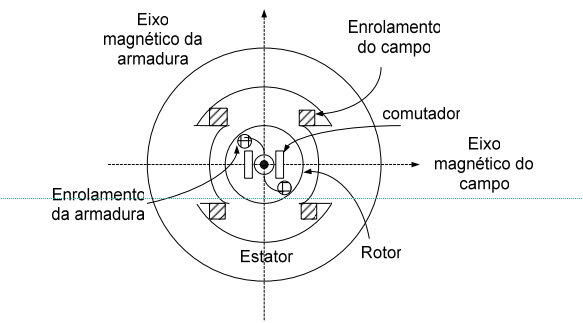
\includegraphics[scale=0.66]{imagens/maquina_cc.png}
\caption{\label{fig:MCC}Máquina de corrente contínua elementar.}
\caption*{Fonte: Máquinas de corrente contínua \protect\footnotemark}
\end{figure}

\footnotetext{Disponível em: <http://www.gsep.ene.unb.br/osem/ivan/Conversao> Acesso em out. 2018.}


\FloatBarrier
\newpage

\section{Motores de Corrente Contínua}


Uma máquina de corrente contínua pode funcionar tanto como um gerador, convertendo energia mecânica em energia elétrica, quanto como um motor, convertendo energia elétrica em mecânica. Apesar de a energia elétrica ser comumente distribuída (no nível do consumidor) em corrente alternada, os motores de corrente contínua possuem grande participação na indústrias, uma vez que permitem facilmente a variação de velocidade, por exemplo, de uma esteira ou um comboio. 

Por outro lado, componentes eletrônicos de tensão alternada, cada vez mais acessíveis, são capazes de controlar a velocidade de motores assíncronos da mesma forma, logo, pelo seu melhor custo benefício, eles vêm substituindo os motores de corrente contínua na maior parte das aplicações. De toda forma, o estudo dos motores de corrente contínua é fundamental pois introduz os conceitos básicos do funcionamento de máquinas elétricas. A figura \ref{fig:MCC} mostra esquematicamente uma máquina de corrente contínua elementar.

\begin{figure}[ht!]
\center
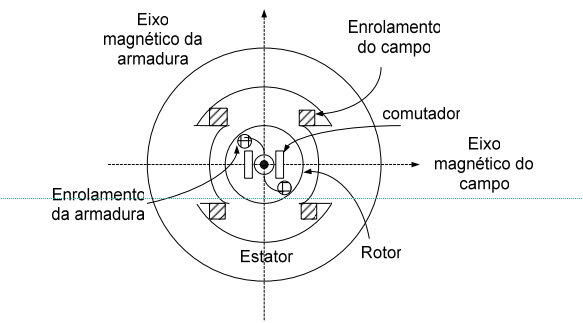
\includegraphics[scale=0.66]{imagens/maquina_cc.png}
\caption{\label{fig:MCC}Máquina de corrente contínua elementar.}
\caption*{Fonte: Máquinas de corrente contínua \protect\footnotemark}
\end{figure}

\footnotetext{Disponível em: <http://www.gsep.ene.unb.br/osem/ivan/Conversao> Acesso em out. 2018.}



\subsection{Comportamento em regime permanente}

\subsubsection{Modelo}

Pode-se ver nas figuras \ref{fig:C11} e \ref{fig:G1_11} o circuito e o gráfico, resp., do modelo de um motor de corrente contínua.

\begin{figure}[ht!]
\center
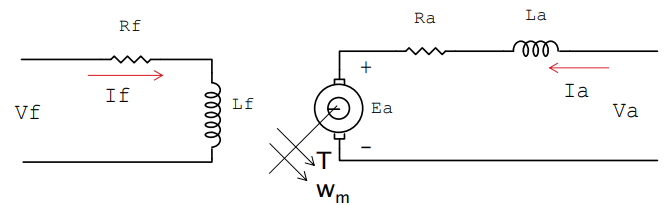
\includegraphics[scale=0.77]{imagens/circuito_11.png}
\caption{\label{fig:C11}Circuito elétrico do modelo geral.}
\caption*{Fonte: MARTINS, cap. 1, eslaide 4.}
\end{figure}

\begin{figure}[ht!]
\center
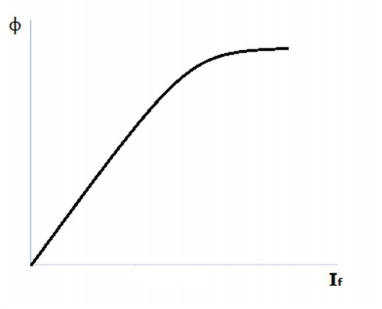
\includegraphics[scale=0.66]{imagens/grafico1_11.png}
\caption{\label{fig:G1_11}Curva de magnetização.}
\caption*{Fonte: MARTINS, cap. 1,  eslaide 4.}
\end{figure}

Partindo da curva de magnetização, podemos caracterizar completamente um motor CC através das equações

\[I_{f} = \frac{V_{f}}{R_{f}}\]

\[V_{a} = R_{a}I_{a} + E_{a}\]
\[E_{a} = k_{a}\phi{\omega_{m}}\]
\[T = k_{a}\phi I_{a}.\]

Assumindo que o motor opera na região linear, tem-se
\[\phi = k_{1}I_{f},\]
logo
\[E_{a} = k\omega_{m}I_{f}\]
\[T = kI_{f}I_{a}.\]

\subsubsection{Excitação separada constante e tensão de armadura variável}

Nesse caso, $\frac{\partial I_f}{\partial t} = 0$, logo

\[T = kI_{f}I_{a} = k_{2}I_{a}\]
\[E_{a} = k_{2}\omega_{m}\]
\[V_{a} = R_{a}I_{a} + E_{a} = R_{a}I_{a} + k_{2}\omega_{m}\]
\[\omega_{m} = \frac{V_{a} - R_{a}I_{a}}{k_{2}} = \frac{V_{a}}{k_{2}} - \frac{ R_{a}I_{a}}{k_{2}}.\]

Caso $R_{a} = 0$, $\omega_{m} = \frac{V_{a}}{k_{2}}$.

Diretamente, pode-se ver que a velocidade é diretamente proporcional à tensão de armadura. Entretanto, pela definição de $I_{f}$,

\[I_{a} = \frac{V_{a} - k_{2}\omega_{m}}{R_{a}},\]
logo,
\[T = \frac{k_{2}}{R_{a}}(V_{a} - k_{2}\omega_{m}) = \frac{k_{2}}{R_{a}}V_{a} - \frac{k_{2}}{R_{a}}k_{2}\omega_{m}.\]

Dessa forma, a velocidade do motor ($\omega_m$) pode ser estudada a partir da tensão de armadura (torque), como na figura \ref{fig:G1_12}. O circuito equivalente pode ser observado na figura \ref{fig:C12}.

\begin{figure}[ht!]
\center
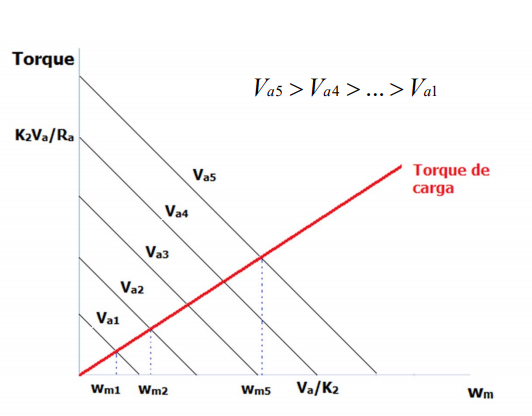
\includegraphics[scale=0.66]{imagens/grafico1_12.png}
\caption{\label{fig:G1_12}Curva Torque-Velocidade para o motor CC com excitação separada constante e tensão de armadura variável}
\caption*{Fonte: MARTINS, cap. 1, eslaide 7.}
\end{figure}


\begin{figure}[ht!]
\center
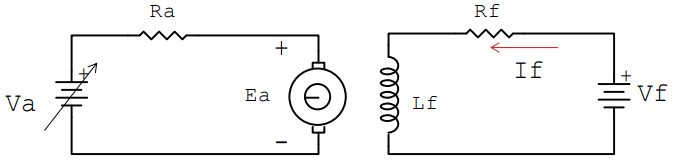
\includegraphics[scale=0.77]{imagens/circuito_12.png}
\caption{\label{fig:C12}Representação na forma de circuito}
\caption*{Fonte: MARTINS, cap. 1, eslaide 7.}
\end{figure}

As máquinas reais, entretanto, possuem $R_{a} \neq 0$, portanto as curvas comportam-se conforme ilustrado na figura \ref{fig:G2_12}.

\begin{figure}[ht!]
\center
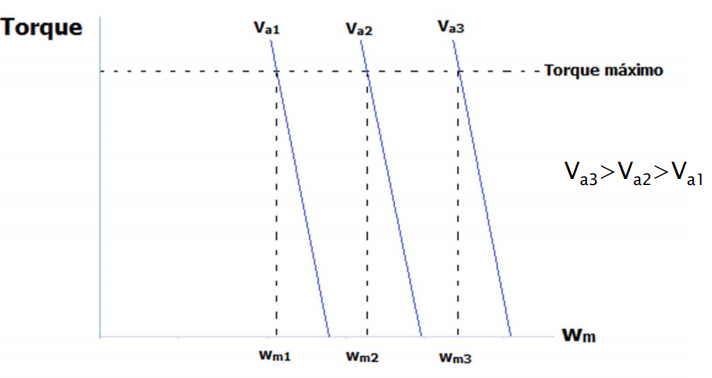
\includegraphics[scale=0.66]{imagens/grafico2_12.png}
\caption{\label{fig:G2_12}Torque em função da velocidade para $R_a \neq 0$}
\caption*{Fonte: MARTINS, cap. 1, eslaide 8.}
\end{figure}

Portanto, limitando $I_{a}$ podemos controlar o torque, uma vez que ele é proporcional à corrente de armadura.

\subsubsection{Excitação separada, corrente de armadura constante e corrente de campo variável}

Neste caso, muito útil quando se deseja motores mais compactos, o circuito é representado na figura \ref{fig:C13}.

\begin{figure}[ht!]
\center
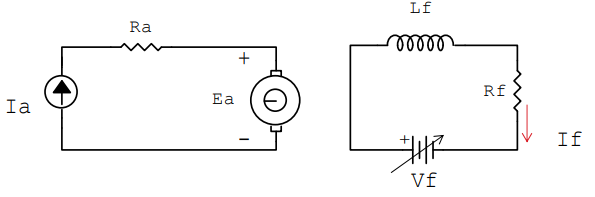
\includegraphics[scale=0.77]{imagens/circuito_13.png}
\caption{\label{fig:C13} Circuito equivalente do motor CC com excitação separada, corrente de armadura constante e corrente de campo variável.}
\caption*{Fonte: MARTINS,2006, eslaide 9.}
\end{figure}

Dado que $I_{a}$ é constante,
\[T = kI_{f}I_{a} = k_{4}I_{f}.\]

Vê-se que o torque não depende da velocidade. O comportamento do torque em função da velocidade é demonstrado na figura \ref{fig:G1_13}.

\begin{figure}[ht!]
\center
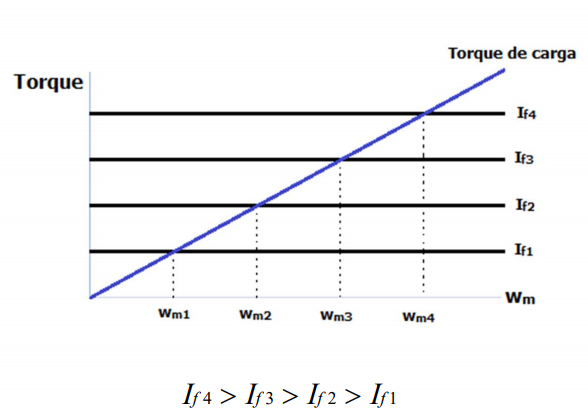
\includegraphics[scale=0.77]{imagens/grafico1_13.png}
\caption{\label{fig:G1_13}Curva Torque-Velocidade do motor CC em excitação separada, corrente de armadura constante e corrente de campo variável.}
\caption*{Fonte: MARTINS, cap. 1, eslaide 10.}
\end{figure}

Aqui, o conversor atua sobre a excitação onde a corrente é menor e a corrente de armadura é constante, o que impede que haja curto-circuito na armadura. Entretanto, o sistema é mais lento pois a constante de tempo mecânica é maior do que a elétrica.

\subsubsection{Excitação separada, tensão de armadura constante e corrente de campo variável}

Tomando como referência o circuito da figura \ref{fig:C14}, temos
\[E_{a} = k\omega_{m}I_{f} = V_{a} - R_{a}I_{a}\]
\[\omega_{m} = \frac{V_{a} - R_{a}I_{a}}{kI_{f}}.\]

\begin{figure}[ht!]
\center
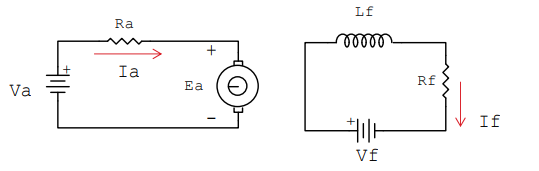
\includegraphics[scale=0.88]{imagens/circuito_14.png}
\caption{\label{fig:C14} Circuito equivalente do motor CC com excitação separada, tensão de armadura constante e corrente de campo variável.}
\caption*{Fonte: MARTINS, cap. 1, eslaide 11.}
\end{figure}

Supondo $R_{a} = 0$, $\omega_{m} = \frac{V_{a}}{kI_{f}} $. Dessa forma, ao atenuar o campo pode-se aumentar a velocidade, ou vice-versa.
\[T = kI_{f}I_{a} = kI_{f} \frac{(V_{a} - E_{a})}{R_{a}}\]
\[T = \frac{kV_{a}}{R_{a}}I_{f} - \frac{kI_{f}}{R_{a}}E_{a}\]
\[T = \frac{kV_{a}}{R_{a}}I_{f} - \frac{k^{2}I_{f}^{2}}{R_{a}}\omega_{m}.\]

I.e., o torque (T) se comporta como na figura \ref{fig:G1_14}.

\begin{figure}[ht!]
\center
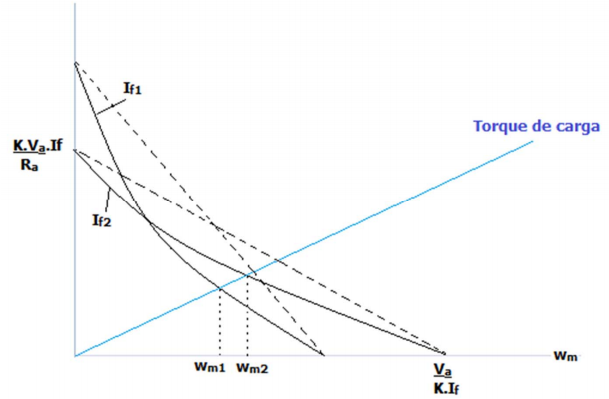
\includegraphics[scale=0.66]{imagens/grafico1_14.png}
\caption{\label{fig:G1_14} Curva Torque-Velocidade do motor CC com excitação separada, tensão de armadura constante e corrente de campo variável.}
\caption*{Fonte: MARTINS, cap. 1, eslaide 12.}
\end{figure}

Note que a diminuição da corrente $I_{f}$ provoca o aumento da velocidade do motor. 

\subsection{Excitação série}
 
A partir do circuito da figura \ref{fig:C15}, tem-se que $I_{f}=I_{a}$, portanto
\[E_{a} = kI_{f}\omega_{m} = kI_{a}\omega_{m}\]
\[V_{a} = R_{a}I_{a} + E_{a} = R_{a}I_{a} + k\omega_{m}I_{a}\]
\[I_{a} = \frac{V_{a}}{R_{a} + k\omega_{m}}\]
\[T = kI_{f}I_{a} = kI_{a}^{2} = \frac{kV_{a}^{2}}{(R_{a} + k\omega_{m})^{2}}.\]
 
\begin{figure}[ht!]
\center
\caption{\label{fig:C15} Circuito equivalente do motor CC com excitação série.}
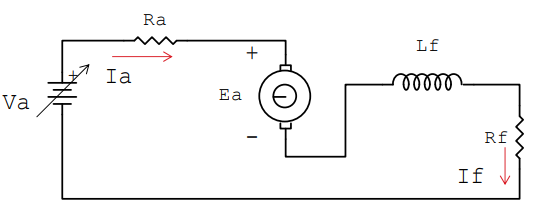
\includegraphics[scale=0.77]{imagens/circuito_15.png}
\caption*{Fonte: MARTINS, cap. 1, eslaide 13.}
\end{figure}


Se $R_{a} = 0$,
\[T = \frac{V_{a}^{2}}{k\omega_{m}^{2}}.\]

A relação torque-velocidade encontra-se representado graficamente na figura \ref{fig:G1_15} para diferentes valores de $V_{a}$.

\begin{figure}[t!]
\center
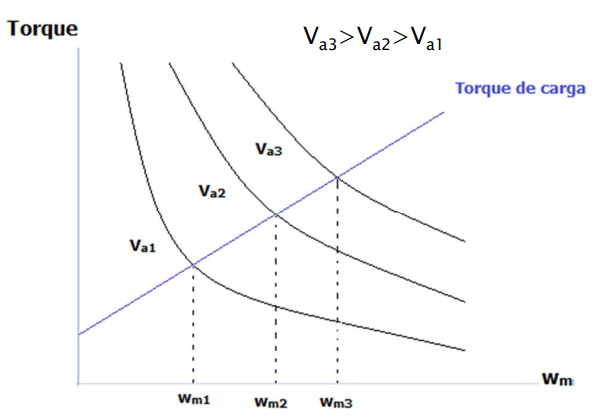
\includegraphics[scale=0.66]{imagens/grafico1_15.png}
\caption{\label{fig:G1_15}Curva Torque-Velocidade do motor CC com excitação série.}
\caption*{Fonte: MARTINS, cap. 1, eslaide 14.}
\end{figure}
 
É possível controlar a velocidade através da variação da tensão de alimentação de armadura.

O motor série oferece, principalmente, um elevado torque de partida. Por isso, ele é tipicamente utilizado em aplicações que necessitam de tração elétrica, além de aplicações de baixa potência.

 
\subsection{Comportamento dinâmico e transitório}

\subsubsection{Modelo completo}

\begin{figure}[ht!]
\center
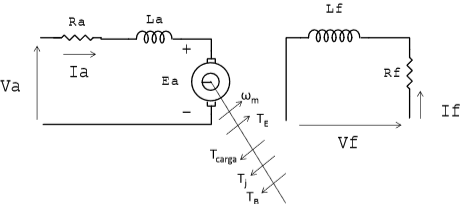
\includegraphics[scale=0.88]{imagens/circuito_31.png}
\caption{\label{fig:C31}Circuito equivalente: excitação separada, corrente de campo constante.}
\caption*{Fonte: MARTINS, cap. 2, eslaide 2.}
\end{figure}

Utilizando como base o motor com excitação separada e corrente de campo constante, como na figura \ref{fig:C31}, tem-se que, para $I_{f}$ constante,
\[V_{a} = R_{a}i_{a} + L_{a}\frac{d i_{a}}{d_{t}} + E_{a}\]
\[E_{a} = K_{e}\omega_{m}\]
\[T_{e} = K_{t}i_{a}\]
\[T_{e} = T_{carga} + J\frac{d\omega_{m}}{d_{t}} + B\omega_{m},\]
onde
\begin{itemize}
   \item $k_{e}$: Constante de velocidade.
   \item $k_{t}$: Constante de armadura.
   \item $R_{a}$, $L_{a}$: Parâmetros de armadura.
   \item B, J : Parâmetros mecânicos.
   \item J: Coeficiente de inércia.
   \item B: Coeficiente de atrito.
\end{itemize}

As equações apresentadas anteriormente modelam o motor sob qualquer alimentação de carga. Portanto, no domínio da frequência complexa,
\[V_{a}(s) = R_{a}i_{a}(s) + SL_{a}i_{a}(s) + K_{e}\omega_{m}(s)\]
\[k_{t}i_{a}(s) = T_{C}(s) + SJ\omega_{m}(s) + B\omega_{m}(s).\]
Dessa forma,
\[V_{a}(s) - k_{e}\omega_{m}(s) = (R_{a} + SL_{a})i_{a}(s)\]
\[i_{a}(s) = \frac{V_{a}(s) - k_{e}\omega_{m}(s)}{(R_{a} + SL_{a})},\]
ou também
 \[i_{a}(s) = \frac{V_{a} - k_{e}\omega_{m}(s)}{(R_{a})}\frac{1}{\left(  s + \frac{1}{\tau_{a}}\right)}.\]
 
Definindo $\tau_{a} = \frac{L_{a}}{R_{a}}$ a constante de tempo de armadura, a figura \ref{fig:D1_31} apresenta um modelo de $i_{a}(s)$ na forma de diagrama de blocos.  
 
\begin{figure}[ht!]
\center
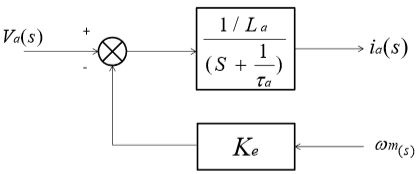
\includegraphics[scale=0.88]{imagens/diagrama1_31.png}
\caption{\label{fig:D1_31}Representação parcial em diagrama de blocos da saída em corrente.}
\caption*{Fonte: MARTINS, cap. 2, eslaide 5.}
\end{figure}

A partir da equação do torque, têm-se
\[\frac{k_{t}i_{a(S) - T_{C}(s)}}{SJ + B} = \omega_{m}(s)\]
ou
\[\omega_{m}(s) = \frac{V_{a} - k_{e}\omega_{m}(s)}{(R_{a})}\frac{1}{\left(s + \frac{1}{\tau_{a}}\right)}.\]

Sendo $\tau_{m} = \frac{J}{B}$ a constante de tempo mecânica, podemos partir da definição de $\omega_{m}$ e obter o diagrama da figura \ref{fig:D2_31}.

\begin{figure}[ht!]
\center
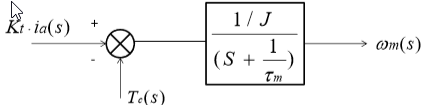
\includegraphics[scale=0.88]{imagens/diagrama2_31.png}
\caption{\label{fig:D2_31} Representação na forma de diagrama de blocos da saída em velocidade.}
\caption*{Fonte: MARTINS, cap. 2, eslaide 6.}
\end{figure}

Com os diagramas das figuras \ref{fig:D1_31} e \ref{fig:D2_31}, pode-se montar o diagrama como na figura \ref{fig:D3_31}.

\begin{figure}[ht!]
\center
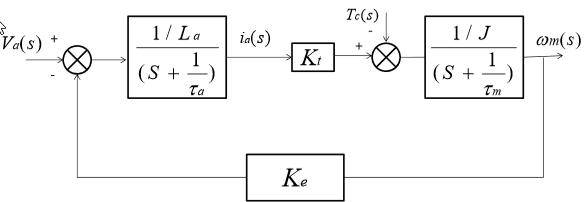
\includegraphics[scale=0.77]{imagens/diagrama3_31.png}
\caption{\label{fig:D3_31}Representação completa na forma de diagrama de blocos do motor CC.}
\caption*{Fonte: MARTINS, cap. 2, eslaide 7.}
\end{figure}

Assim, obtêm-se as funções de transferência para
\[\frac{\omega_{m}(s)}{V_{a}(s)}\]
\[\frac{i_{a}(s)}{V_{a}(s)}.\]

O sistema realimentado como na figura \ref{fig:D4_31} é caracterizado por
\[\frac{C(s)}{R(s)} = \frac{G(s)}{1  \pm G(s)H(s)}.\]

\begin{figure}[ht!]
\center
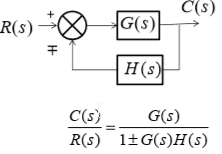
\includegraphics[scale=0.99]{imagens/diagrama4_31.png}
\caption{\label{fig:D4_31} Sistema realimentado representado na forma de diagrama de blocos.}
\caption*{Fonte: MARTINS, cap. 2, eslaide 8.}
\end{figure}

Portanto,
\[\frac{\omega_{m}(s)}{V_{a}(s)} = \frac{\frac{k_{t}}{L_{a}\left(s + \frac{1}{\tau_{a}}\right)J\left(s + \frac{1}{\tau_{m}}\right)}}{1 + \frac{k_{t}k_{e}}{L_{a}J\left(s + \frac{1}{\tau_{a}}\right)\left(s + \frac{1}{\tau_{m}}\right)}}\]

\[\frac{\omega_{m}(s)}{V_{a}(s)} =  \frac{k_{t}}{L_{a}\left[  \left(s + \frac{1}{\tau_{a}}\right)\left(s + \frac{1}{\tau_{m}}\right) + \frac{1}{\tau_{a}\tau_{ml}}\right] } .\]

Dessa forma,
\[\frac{i_{a}(s)}{V_{a}(s)} = \frac{\frac{1}{L_{a}\left(s + \frac{1}{\tau_{a}}\right)}}{1 + \frac{k_{t}k_{e}}{L_{a}J\left(s + \frac{1}{\tau_{a}}\right)\left(s + \frac{1}{\tau_{m}}\right)}},\]
i.e.,
\[\frac{i_{a}(s)}{V_{a}(s)} =  \frac{\left(s + \frac{1}{\tau_{m}}\right)}{L_{a}\left[  \left(s + \frac{1}{\tau_{a}}\right)\left(s + \frac{1}{\tau_{m}}\right) + \frac{1}{\tau_{a}\tau_{ml}}\right] } \] 
uma vez que $\tau_{ml} = \frac{R_{a}.J}{k_{e}.k_{t}}$.

\subsubsection{Modelo simplificado}

Considerando a indutância $L_{a}=0$, a configuração pode assumir a lógica do diagrama de blocos ilustrado na figura \ref{fig:D1_32} 

\begin{figure}[ht!]
\center
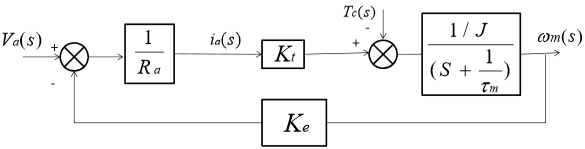
\includegraphics[scale=0.77]{imagens/diagrama1_32.png}
\caption{\label{fig:D1_32} Representação do modelo simplificado em diagrama de blocos.}
\caption*{Fonte: MARTINS, cap. 2, eslaide 10.}
\end{figure}

Dado que o torque $T_{c}$ é nulo, tem-se \[
    \frac{\omega_{m}(s)}{V_{a}(s)} = \frac{\frac{k_{t}}{R_{a}J\left(s + \frac{1}{\tau_{m}}\right)}}{1 + \frac{k_{t}k_{e}}{R_{a}J\left(s + \frac{1}{\tau_{m}}\right)}} \Rightarrow \frac{\omega_{m}(s)}{V_{a}(s)} = \frac{\frac{k_{t}}{R_{a}J}}{\left(s + \frac{1}{\tau_{m}}\right) + \frac{k_{t}k_{e}}{R_{a}J} }
\] ou
\[\frac{\omega_{m}(s)}{V_{a}(s)} = \frac{k_{t}}{R_{a}J}\frac{1}{\left[  \left(s + \frac{1}{\tau_{m}}\right) + \frac{k_{t}k_{e}}{R_{a}J}\right] }\]
\[\frac{1}{\tau_{m}} + \frac{k_{t}k_{e}}{R_{a}J} = \frac{1}{\tau_{m}} + \frac{1}{\tau_{ml}} = \frac{\tau_{m} + \tau_{ml}}{\tau_{m}\tau_{ml}} = \frac{1}{k\tau_{ml}}\]

Uma vez que $ K = \frac{\tau_{m}}{\tau_{m} + \tau_{ml}}$ 

\[\frac{\omega_{m}(s)}{V_{a}(s)} = \frac{k_{t}}{R_{a}J}\frac{1}{\left(s + \frac{1}{K\tau_{ml}}\right)} .\]



\subsection{Regulação de velocidade e de corrente}

Usualmente, motores alimentados por retificadores ou conversores CC-CC podem ter sua velocidade e corrente controladas. Com isso, é possível obter maior precisão no controle de velocidade, melhor resposta dinâmica, menor sensibilidade a variações de torque da carga, controle da corrente máxima nos semicondutores de potência e no motor e também a limitação no torque máximo produzido pelo motor e na aceleração máxima na carga.

\subsubsection{Modelo do motor e do conversor}

A figura \ref{fig:C1_42} apresenta o circuito equivalente do motor CC.

\begin{figure}[ht!]
\center
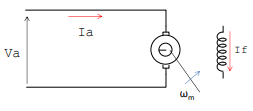
\includegraphics[scale= 1]{imagens/circuito1_42.png}
\caption{\label{fig:C1_42}Circuito equivalente motor CC.}
\caption*{Fonte: MARTINS, cap. 2, eslaide 13.}
\end{figure}

Para esse circuito, se aplica a função de transferência conforme no diagrama da figura \ref{fig:DBMCC}.

\begin{figure}[ht!]
\center
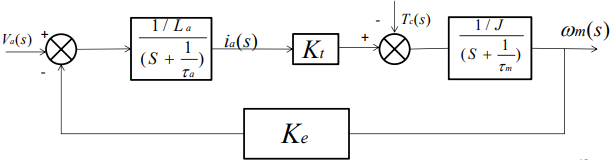
\includegraphics[scale= 0.88]{imagens/diagrama1_42.png}
\caption{\label{fig:DBMCC}Diagrama de blocos do motor CC.}
\caption*{Fonte: MARTINS, cap. 2, eslaide 13.}
\end{figure}

Levando $T_{C}(s)$ a zero na figura \ref{fig:D1_42}, obtém-se 
\[\frac{\omega_{m}(s)}{V_{a}(s)} =  \frac{k_{t}}{L_{a}J\left[\left(s + \frac{1}{\tau_{a}}\right)\left(s + \frac{1}{\tau_{m}}\right) + \frac{1}{\tau_{a}\tau_{ml}}\right] }.\]
I.e., a figura \ref{fig:D2_42} representa o funcionamento do motor.

\begin{figure}[ht!]
\center
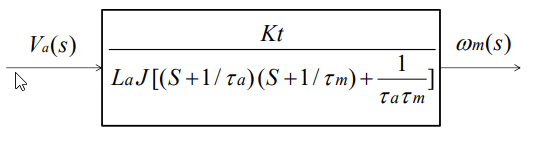
\includegraphics[scale= 0.88]{imagens/diagrama2_42.png}
\caption{\label{fig:D2_42}Diagrama de blocos compactado do motor CC.}
\caption*{Fonte: MARTINS, cap. 2, eslaide 14.}
\end{figure}

Sabendo que a condução do conversor é contínua e ignorando o atraso induzido pelo mesmo, tem-se a representação em diagrama de blocos conforme na figura \ref{fig:D3_42}, cuja função de transferência é 
\[\frac{V_{a}(s)}{E_{c}(s)} = k_{c}.\]
Portanto, a função de transferência do conjunto conversor-motor será como ilustrado na figura \ref{fig:D1_42}.

\begin{figure}[ht!]
\center
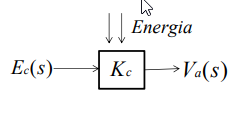
\includegraphics[scale= 0.88]{imagens/diagrama3_42.png}
\caption{\label{fig:D3_42}Representação idealizada do conversor estático que alimenta o motor CC.}
\caption*{Fonte: MARTINS, cap. 2, eslaide 15.}
\end{figure}

\begin{figure}[ht!]
\center
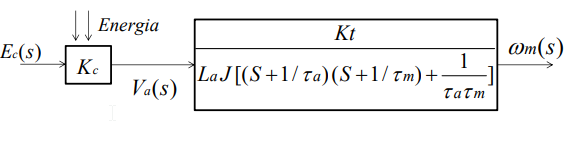
\includegraphics[scale= 0.88]{imagens/diagrama4_42.png}
\caption{\label{fig:D1_42} Diagrama de blocos do conversor alimentando o motor CC.}
\caption*{Fonte: MARTINS, cap. 2, eslaide 15.}
\end{figure}

\subsubsection{Regulação de velocidade}

Quando se realiza um sensor de velocidade e um regulador de velocidade, o controle de velocidade em malha fechada é viável. Nesse caso, o diagrama de blocos é conforme ilustrado na figura \ref{fig:D1_43}.

\begin{figure}[ht!]
\center
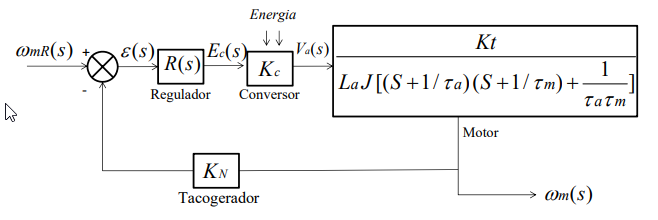
\includegraphics[scale= 0.88]{imagens/diagrama1_43.png}
\caption{\label{fig:D1_43} Diagrama de blocos do conjunto motor CC e conversor estático com regulador de velocidade.}
\caption*{Fonte: MARTINS, cap. 2, eslaide 16.}
\end{figure} 
 
Um regulador proporcional, regido por
 \[R(s) = k_{R}\]
não altera a ordem do sistema e possui um erro de posição inversamente proporcional ao ganho do regulador.
 
Já um regulador proporcional-integral, de forma
\[R(s) = k_{R}\frac{\left(1+s+\tau_{R}\right)}{s\tau_{R}}\]
possui erro de posição nulo e maior precisão estática no controle, sendo que $k_{R}$ pode assumir valores menores do que no caso puramente proporcional.

\subsubsection{Regulação de corrente}

Com um erro de velocidade grande, o sistema de controle resulta em valores altos de corrente de armadura. A função de transferência é representada na figura \ref{fig:D1_44}. Pode-se representar um regulador de corrente como na figura \ref{fig:D2_44}.

\begin{figure}[ht!]
\center
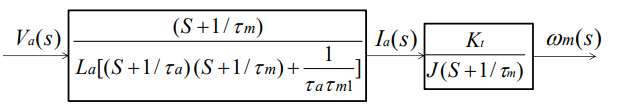
\includegraphics[scale= 0.88]{imagens/diagrama1_44.png}
\caption{\label{fig:D1_44}Outra forma de representar o motor CC em diagrama de blocos.}
\end{figure} 

\begin{figure}[ht!]
\center
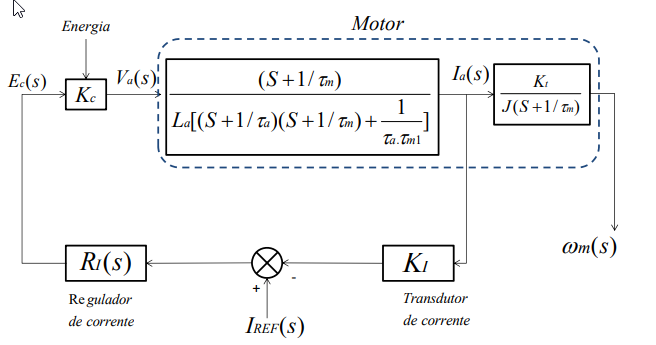
\includegraphics[scale= 0.88]{imagens/diagrama2_44.png}
\caption{\label{fig:D2_44}Diagrama de blocos do  motor CC e conversor estático com regulador de corrente.}
\caption*{Fonte: MARTINS, cap. 2, eslaide 19.}
\end{figure} 

Aqui, $R_{l}(s)$ representa o regulador de corrente. Também é possível implementar para tal um regulador proporcional ou um proporcional-integral. A limitação de $I_{a}(s)$ é dada pelo limite do valor máximo da corrente de referência $I_{REF}(s)$.

Caso ambos os reguladores de velocidade e de corrente sejam utilizados, basta limitar o erro de velocidade para limitar $I_{a}(s)$, como ilustra a figura \ref{fig:D3_44}. Esse método é conhecido como regulação em cascata.

\begin{figure}[ht!]
\center
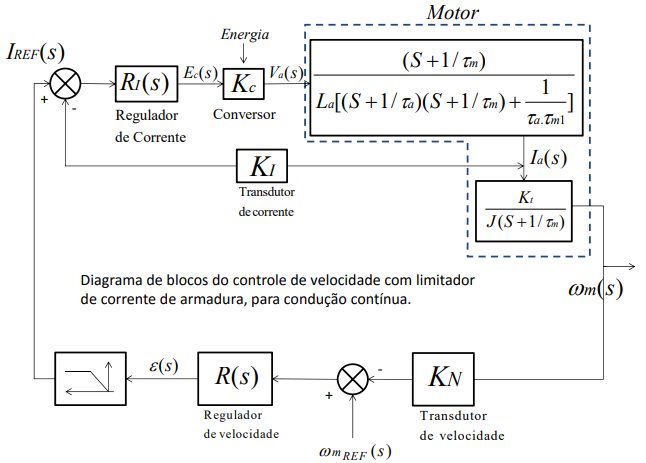
\includegraphics[scale= 0.88]{imagens/diagrama3_44.png}
\caption{\label{fig:D3_44}Diagrama de blocos do controle de velocidade com limitador de corrente de armadura, para condução contínua.}
\caption*{Fonte: MARTINS, cap. 2, eslaide 21.}
\end{figure} 

\subsubsection{Monitoração da velocidade}

Uma forma de monitorar a velocidade é através da força eletromotriz produzida pelo motor, como ilustra a figura \ref{fig:C1_45}). Considerando uma excitação constante,
\[E_{a} = k_{a}\omega_{m} = V_{m} - R_{a}I_{a}.\]

\begin{figure}[ht!]
\center
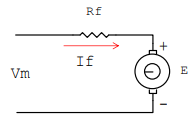
\includegraphics[scale= 0.88]{imagens/circuito_45.png}
\caption{\label{fig:C1_45} Método da força eletromotriz.}
\caption*{Fonte: MARTINS, cap. 2, eslaide 22.}
\end{figure} 

Na figura \ref{fig:C2_45} pode-se obter o valor de $E_{a}$ e da corrente (resistor em série com a a armadura). Logo, a tensão proporcional do motor é obtida simplesmente na saída do amplificador.

\begin{figure}[ht!]
\center
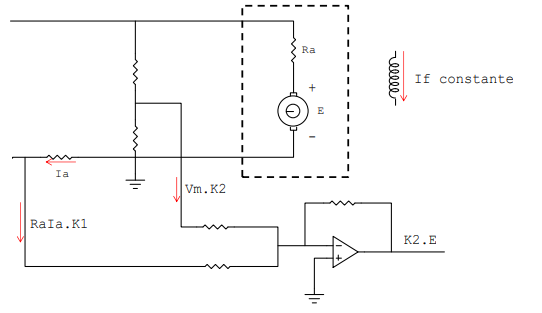
\includegraphics[scale= 0.88]{imagens/circuito2_45.png}
\caption{\label{fig:C2_45} Medida indireta da força eletro-motriz.}
\caption*{Fonte: MARTINS, cap. 2, eslaide 23.}
\end{figure} 

Uma outra forma de monitorar a velocidade é usando um tacogerador, que fornece maior precisão no controle de velocidade pois possui excelente linearidade. Esse método produz ruídos com frequência e amplitude proporcionais à velocidade. No caso de velocidades baixas, onde o uso de filtros interfere na resposta do sistema, emprega-se tacogeradores de grande diâmetro com muitas lâminas no comutador. Tacogeradores digitas são ainda mais precisos do que os de tensão contínua.

\subsubsection{Sensores de corrente}

Uma abordagem para o monitoramento de corrente é utilizando transdutores de corrente alternada, utilizando-se um transformador de corrente no lugar de corrente alternada do conversor, como ilustra a figura \ref{fig:C1_46}. Veja que esse método não é aplicável na presença de um diodo de roda livre.

\begin{figure}[ht!]
\center
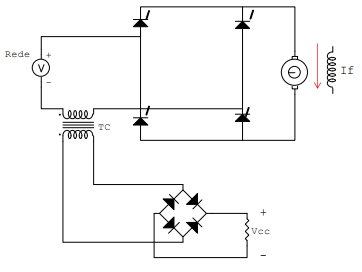
\includegraphics[scale= 0.88]{imagens/circuito1_46.png}
\caption{\label{fig:C1_46}Uso de transformador de corrente no lado CA do conversor.}
\caption*{Fonte: MARTINS, cap. 2, eslaide 25.}
\end{figure} 

A abordagem mais econômica é através de um sensor resistivo, apesar da tensão de nível ser muito baixa. Além disso, o sinal não é eletricamente isolado da parte de potência, o que é uma desvantagem.

Já o transdutor magnético de corrente contínua produz um resistência $R$ proporcional à corrente $I_{a}$. Seu princípio é ilustrado na figura \ref{fig:C2_46}.

\begin{figure}[ht!]
\center
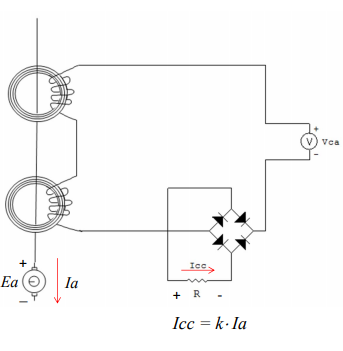
\includegraphics[scale= 0.88]{imagens/circuito2_46.png}
\caption{\label{fig:C2_46} Transdutor magnético de corrente contínua.}
\caption*{Fonte: MARTINS, cap. 2, eslaide 27.}
\end{figure} 

São aplicados núcleos toroidais de Permalloy, uma liga de ferro-níquel que possui poucas perdas magnéticas e uma permeabilidade alta.

Por fim, é possível também utilizar um transdutor eletrônico CC. O diagrama de blocos da figura \ref{fig:D1_46} demonstra o princípio de funcionamento dessa abordagem.

\begin{figure}[ht!]
\center
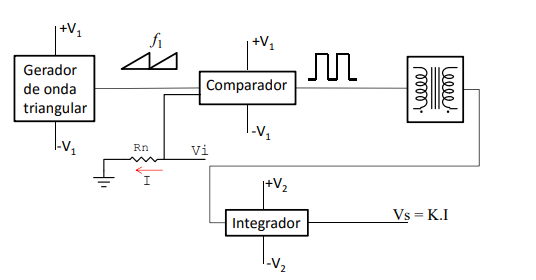
\includegraphics[scale= 0.88]{imagens/diagrama1_46.png}
\caption{\label{fig:D1_46} Transdutor eletrônico de corrente contínua.}
\caption*{Fonte: MARTINS, cap. 2, eslaide 28.}
\end{figure}

$V(s)$ é proporcional ao valor médio da corrente $I$. As fontes $V_{1}$ e $V_{2}$ são isolados entre si. Dessa forma $V_{s}$ também é isolado de $V_{i}$. Por possuir uma frequência $f_{t}$ elevada, esse transdutor possui uma resposta muito rápida. Além disso, é eletronicamente simples e compacto. Vários conversores comerciais possuem esse transdutor.

Um outro tipo de sensor disponível são os sensores a efeito Hall, que apresentam excelente precisão, mas alto custo e difícil implementação (figura \ref{fig:F1_46}).
\[V_{H} = KBI.\]

\begin{figure}[ht!]
\center
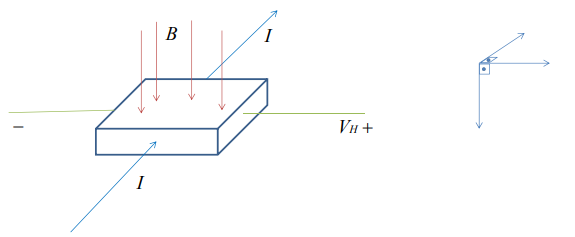
\includegraphics[scale= 0.88]{imagens/figura1_46.png}
\caption{\label{fig:F1_46} Semicondutor submetido a uma indução magnética B e percorrido por uma corrente i}
\caption*{Fonte: MARTINS, cap. 2, eslaide 30.}
\end{figure}

\subsubsection{Reguladores em paralelo}

Em um sistema de regulação em cascata, geralmente é difícil atingir um comportamento dinâmico ótimo, uma vez que dois reguladores influenciam ao mesmo tempo. Assim, costumeiramente utilizam-se os reguladores em paralelo, como ilustra a figura \ref{fig:D1_47}.

\begin{figure}[ht!]
\center
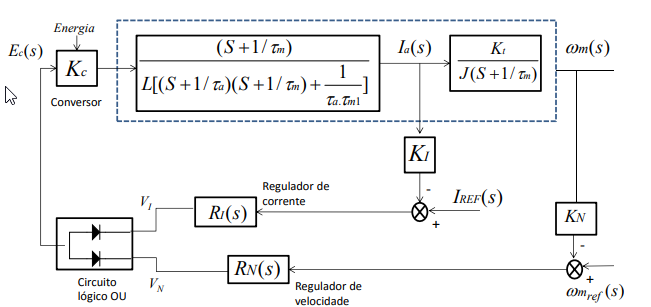
\includegraphics[scale= 0.88]{imagens/diagrama1_47.png}
\caption{\label{fig:D1_47} Motor de corrente contínua controlado por regulador em paralelo.}
\caption*{Fonte: MARTINS, cap. 2, eslaide 32.}
\end{figure}



\subsection{Projeto de reguladores em cascata}
 
\subsubsection{Malha de corrente}

A figura \ref{fig:D1_51} apresenta a malha de regulação de corrente.

\begin{figure}[ht!]
\center
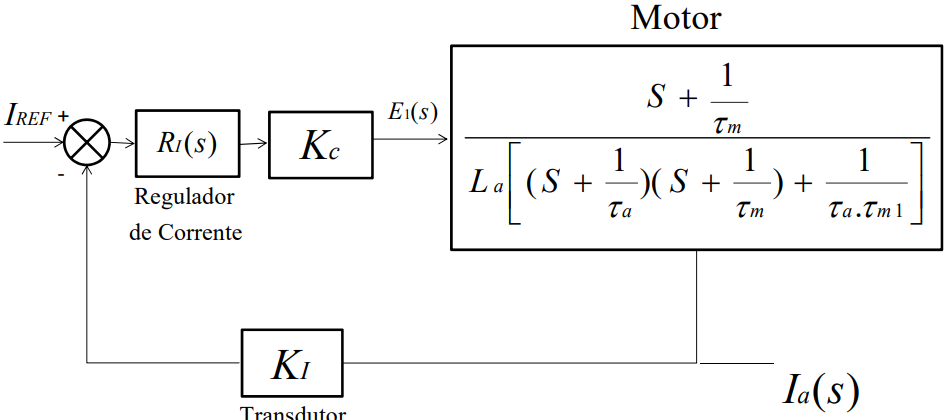
\includegraphics[scale= 0.55]{imagens/diagrama1_51.png}
\caption{\label{fig:D1_51} Malha de regulação de corrente.}
\caption*{Fonte: MARTINS, cap. 3, eslaide 2.}
\end{figure}

Sendo um regulador de corrente proporcional,

$R_{l}(s) = K_{l}; \tau_{l} = \frac{R_{a}J}{K_{e}K_{t}}$.

Para os estudos realizados a seguir considera-se que $\tau_{a} << \tau_{m}$, então $\tau_{a}$ pode ser desprezado em relação a $\tau_{m}$.

Dessa forma o modelo do motor é representado pela seguinte função:

\[\frac{I_{a}(s)}{E_{l}} = \frac{\left(\tau_{m}s + 1\right)}{\left(\frac{L_{a}}{\tau_{a}}\right)\left[\left(1 + s\tau_{a}\right)\left(1 + s\tau_{m}\right) + \left(\frac{\tau_{m}}{\tau_{ml}}\right)\right]}\]

Onde, $\frac{L_{a}}{\tau_{a}} = R_{a}$. Assim:

\[\frac{I_{a}(s)}{E_{l}} = \frac{\left(\tau_{m}s + 1\right)}{R_{a}\left[\left(1 + s\tau_{m}\right) + \left(\frac{\tau_{m}}{\tau_{ml}}\right)\right]}\]

\[1 +s\tau_{m} + \frac{\tau_{m}}{\tau_{ml}} = \tau_{m}\left(s + \frac{1}{\tau_{m}} +\frac{1}{\tau_{ml}}\right) = \tau_{m}\left[s + \frac{\left(\tau_{m} + \tau_{ml}\right)}{\tau_{m}\tau_{ml}}\right] = \frac{\tau_{m} + \tau_{ml}}{\tau_{ml}}\left(1 + s\frac{\tau_{m}\tau_{ml}}{\tau_{m} + \tau_{ml}}\right)\]

Seja $K_{1} = \frac{\tau_{m1}}{R_{a}\left(\tau_{m} + \tau_{m1}\right)} = \frac{D}{K_{e}^{2} + DR{a}}$ e $\tau_{m2} = \frac{\tau_{m}\tau_{m1}}{\tau_{m} + \tau_{m1}}$

Onde, $D = \frac{J}{\tau_{m}}$

Assim:
\[\frac{I_{a}(s)}{E_{1}(s)} = K_{1}\frac{\left(1 + s\tau_{m}\right)}{1 + s\tau_{m2}} \]

Dessa forma, o diagrama de blocos é representado pela figura \ref{fig:D2_51}.

\begin{figure}[ht!]
\center
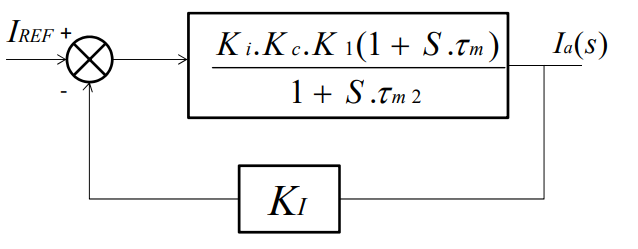
\includegraphics[scale= 0.55]{imagens/diagrama2_51.png}
\caption{\label{fig:D2_51} Diagrama de blocos do motor CC com regulador de corrente.}
\caption*{Fonte: MARTINS, cap. 3, eslaide 4.}
\end{figure}

Logo:
\[\frac{I_{a}(s)}{I_{REF}(s)} = \frac{K_{i}K_{e}K_{1}\frac{\left(1 + s\tau_{m}\right)}{1 + s\tau_{m2}}}{1 + K_{i}K_{c}K_{1}K_{I}\frac{1 + s\tau_{m}}{1 + s\tau_{m2}}}\]

Assim:
\[\frac{I_{a}(s)}{I_{REF}(s)} = \frac{K_{i}K_{c}K_{1}\left(1 + s\tau_{m}\right)}{\left(1 + s\tau_{m2}\right) + K_{i}K_{c}K_{1}\left(1 + s\tau_{m}\right)}\]

\[\frac{I_{a}(s)}{I_{REF}(s)} = \frac{K_{i}K_{c}K_{1}\left(1 + s\tau_{m}\right)}{\left(1 + K_{i}K_{c}K_{1}K_{1}\right) + \left[1 + s\left(\frac{\tau_{m2} + K_{i}K_{c}K_{1}K_{I}\tau_{m} }{1 + K_{i}K_{c}K_{1}K_{I}}\right)\right]}\]

Seja um $K_{i}$ escolhido de modo que $K_{i}.K_{c}.K_{1}.K_{I} >> 1$. Assim:

\[\frac{I_{a}(s)}{I_{REF}(s)} = \frac{K_{i}K_{c}K_{1}\left(1 + s\tau_{m}\right)}{ K_{i}K_{c}K_{1}\left(1 + s\tau_{m3}\right)}\]

Onde, $\tau_{m3} = \frac{\tau_{m2}}{K_{i}K_{c}K_{1}K_{I}} + \tau_{m}$

Um $K_{i}$ grande, além de diminuir o erro estático, torna $\tau_{m3} = \tau_{m}$ o que implica no cancelamento pólo-zero da malha. Assim:

\[\frac{I_{a}(s)}{I_{REF}(s)} \frac{1}{K_{I}}\]

Desse modo, para se limitar a corrente de armadura do motor, basta limitar a corrente de referência $I_{REF}(s)$. 

\subsubsection{Ganho do regulador de corrente e o erro estático}

Dado que a equação a seguir define o erro estático relativo:
\[\epsilon_{R} = \frac{I_{REF} - K_{I}I_{a}}{I_{REF}}  \]


É possível provar que:
\[K_{i} = \frac{1 - \epsilon_{R}}{\epsilon_{R}}K_{c}K_{1}K_{I}\]

\subsubsection{Malha de velocidade}

O diagrama de blocos ilustrado na figura \ref{fig:D1_53} representa a malha de velocidade.

\begin{figure}[ht!]
\center
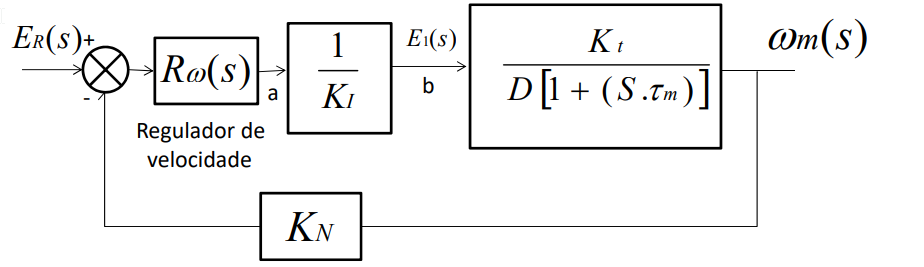
\includegraphics[scale= 0.55]{imagens/diagrama1_53.png}
\caption{\label{fig:D1_53} Diagrama de blocos para estudo da malha de velocidade.}
\caption*{Fonte: MARTINS, cap. 3, eslaide 7.}
\end{figure}

Onde, $D = \frac{J}{\tau_{m}}$
Seja um controlador proporcional integral para a velocidade. Assim:
\[R_{w}(s) = 	\left ( A + \dfrac{B}{s} \right ) = \frac{As + B}{s} = \frac{\left(1 + \frac{A}{B}s\right)}{\frac{s}{B}}\]

\[R_{w}(s) = A \frac{\left(1 + \frac{A}{B}s\right)}{\frac{A}{B}s} = \frac{A\left(1 + \tau_{c}s\right)}{s\tau_{c}}\]

Onde:
\[\tau_{c} = \frac{A}{B}\]

Portanto, a figura \ref{fig:D2_53} ilustra o diagrama de blocos conforme as equações anteriores.

\begin{figure}[ht!]
\center
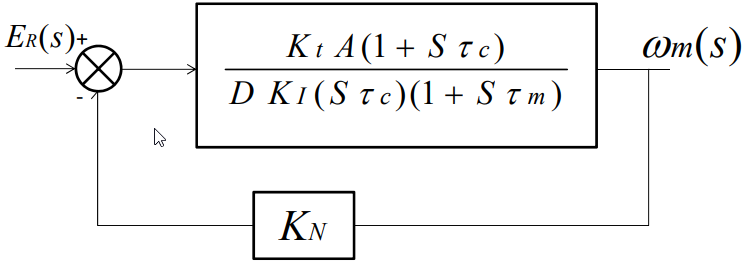
\includegraphics[scale= 0.55]{imagens/diagrama2_53.png}
\caption{\label{fig:D2_53} Estudo da malha de velocidade usando regulador proporcional-integral.}
\caption*{Fonte: MARTINS, cap. 3, eslaide 8.}
\end{figure}

Portanto:

\[\frac{\omega_{m}(s)}{E_{R}(s) } =  \frac{\left(\frac{K_{t}A}{DK_{I}}\frac{\left(1 + \tau_{c}s\right)}{s\tau_{C}\left(1 + s\tau_{m}\right)}\right)}{\left[1 + \left(\frac{K_{t}AK_{N}}{DK_{I}}\frac{\left(1 + \tau_{c}s\right)}{s\tau_{c}\left(1 + s\tau_{m}\right)}\right)\right]}\]

Assim:
 
\[\frac{\omega_{m}(s)}{E_{R}(s) } = \frac{K_{t}A\left(1 + s\tau_{c}\right)}{DK_{t}s\tau_{c}\left(1 + s\tau_{M} + K_{t}AK_{N}\left(1 + s\tau_{c}\right)\right)}\]

\[\frac{\omega_{m}(s)}{E_{R}(s) } = \frac{\frac{1 + s\tau_{c}}{K_{N}}}{1 + \tau_{c}\left(1 + \frac{DK_{I}}{K_{t}K_{N}A}\right)s + \frac{DK_{I}\tau_{c}\tau_{m}}{K_{t}AK_{N}}s^{2} }\]

Seja:
\[\frac{K_{t}AK_{N}}{K} >> 1\]

Portanto:
\[\frac{\omega_{m}(s)}{E_{R}(s) } = \frac{\left(1 + s\tau_{c}/K_{N}\right)}{1 + s\tau_{c} + s^{2}\tau_{c}\tau_{2}}\]

\[ \tau_{2} = \frac{DK_{I}\tau_{m}}{K_{t}K_{N}A}\]

Os pólos da função de transferência são obtidos do seguinte modo:

\[1 + s\tau_{c} + \tau_{c}\tau_{2}s^{2} = 0\]

\[ s^{2} + \frac{1}{\tau_{2}}s + \frac{1}{\tau_{2}\tau_{c}} = 0\]

\[s_{1},s_{2} = \frac{\frac{-1}{\tau_{2}} \pm \sqrt{\frac{1}{\tau_{2}^{2}} - \frac{4}{\tau_{2}\tau_{c}}}}{2}\]

Desta forma:

\[s_{1},s_{2} = \frac{-1}{2\tau_{2}} \pm j\frac{1}{2}\sqrt{\frac{4}{\tau_{2}\tau_{c}}}\sqrt{1 - \frac{\tau_{c}}{4\tau_{2}}}\]

\[s_{1},s_{2} = -\epsilon\omega_{n} \pm j\omega_{n}\sqrt{1 - \epsilon^{2}}\]

Dado que :

$\omega_{n}$ =  Frequência natural não amortecida

$\epsilon$ = Fator de amortecimento relativo


Na prática: $\epsilon = 0,707$
Portanto:
\[\tau_{c} = 2\tau_{2}\]
\[\omega_{n} = \frac{1}{\tau_{2}\sqrt{2}}\]

Escolhendo-se $\omega_{n}$ pode-se obter $\tau_{2}$ e $\tau_{c}$. Sabendo o valor de $\tau_{2}$, pode-se obter A com a seguinte expressão:

\[A = \frac{DK_{I}\tau_{m}}{K_{I}K_{N}\tau_{2}} = \frac{K_{I}J}{K_{t}K_{N}\tau_{2}}\]

Dessa forma os parâmetros do regulador $P_{I}$ podem ser determinados.

Exemplo de cálculo:

Seja um motor CC de 3 HP, 125 V, 1750 rpm, com os seguintes valores:

$R_{a} = 0,6 \Omega$ 

$L_{a} = 0,006 H$

$J = 0,093 Kgm^{2}$ (máquina mais carga)

$D = 0,008 Nm/rad/s$

$K_{t} = K_{c} = 0,6 V/rad/s$

É adicionado externamente um indutor com os seguintes parâmetros:

$L_{ext} = 0,04H$
$R_{ext} = 0,4\Omega$

Desse modo, aplicando-se as equações já desenvolvidas no estudo teórico feito anteriormente obtém-se:

\[\tau_{a} = \frac{L_{a}}{R_{a}} = \frac{0,04 + 0,006}{0,4 + 0,6} = 0,046 seg\]
\[\tau = \frac{J}{D} = \frac{0,093}{0,008} = 11,63 seg\]

Os dados adicionais do problema são apresentados a seguir:

$K_{N} = 0,57 V/rad/s  \rightarrow $ Sensor de velocidade (tacogerador)

$K_{t} = 0,5 V/A  \rightarrow$ Transdutor de corrente.

$K_{C} = 25  \rightarrow$ Ganho do conversor.

Logo, tem-se que:

\[I_{a} = \frac{3.746}{125} = 18A\]
\[\frac{I_{a}}{I_{REF}} = \frac{1}{K_{I}} \rightarrow I_{REF} = 0,5.18 = 9 V \]

Seja $\omega_{n} = 10 rad/seg$ (frequência natural não amortecida). Então:
\[\tau_{2} \frac{1}{\omega_{n}\sqrt{2}}\]
\[\tau_{c} = 2\tau_{2}\]
\[\tau_{2} 0,07 seg\]
\[\tau_{c} = 0,14 seg\]

\[A = \frac{K_{I}J}{K_{t}K_{N}\tau_{2}} = \frac{0,5.0,093}{0,6.0,57.0,07} = 1,94\]
\[\tau_{c} = \frac{A}{B}\]

\[B = \frac{A}{\tau_{c}} = \frac{1,94}{0,14} = 13,86 \]


 
\subsection{Projeto de reguladores em paralelo}

\subsubsection{Malha de corrente}

O estudo da malha de corrente para esta situação é o mesmo para o caso do controle em cascata esboçado na seção anterior.

\subsubsection{Malha de velocidade}

A malha de velocidade pode ser representada pelo diagrama da figura \ref{fig:D1_62}. Dado que $L_{a} = 0$ (pequenas perturbações).

\begin{figure}[ht!]
\center
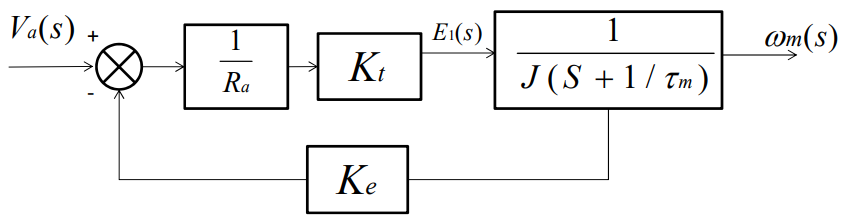
\includegraphics[scale= 0.55]{imagens/diagrama1_62.png}
\caption{\label{fig:D1_62} Diagrama de blocos do motor da malha de velocidade considerando $L_{a} = 0$.}
\caption*{Fonte: MARTINS, cap. 3, eslaide 14.}
\end{figure}

Assim:
\[\frac{\omega_{m}(s)}{V_{a}(s)} = \frac{K_{t}/R_{a}J}{\left(s + 1/\tau_{m2}\right)}\]
\[\tau_{m2} = \frac{\tau_{m1}\tau_{m}}{\tau_{m1} + \tau_{m}}\]
\[\tau_{m1} = \frac{R_{a}J}{K_{e}K_{t}}\]

Portanto, o diagrama de blocos pode ser representado como na figura \ref{fig:D2_62}.

\begin{figure}[ht!]
\center
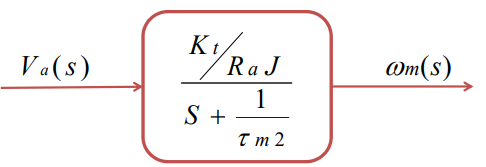
\includegraphics[scale= 0.55]{imagens/diagrama2_62.png}
\caption{\label{fig:D2_62} Diagrama de blocos do motor}
\caption*{Fonte: MARTINS, cap. 3, eslaide 15.}
\end{figure}

A figura \ref{fig:D3_62} representa o diagrama com o conversor e o regulador proporcional - integral inclusos.

\begin{figure}[ht!]
\center
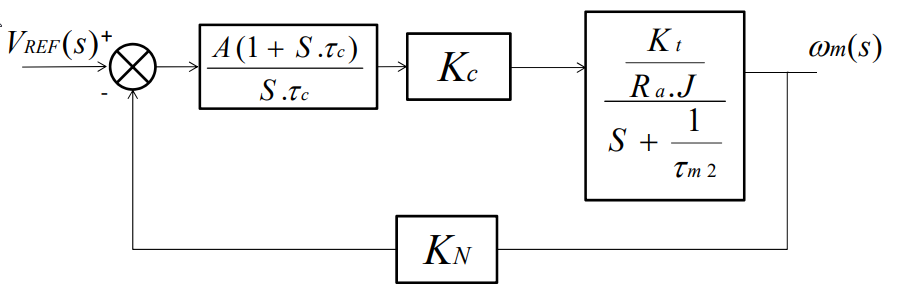
\includegraphics[scale= 0.55]{imagens/diagrama3_62.png}
\caption{\label{fig:D3_62} Diagrama de blocos do motor CC incluindo o conversor estático e o regulador.}
\caption*{Fonte: MARTINS, cap. 3, eslaide 16.}
\end{figure}

A função de transferência é representada pela seguinte expressão:

\[\frac{\omega_{m}(s)}{V_{REF}(s)} = \frac{1 + s\tau_{C}/K_{N}}{1 + s\tau_{C}\left(1 + \frac{R_{a}J}{A.K_{C}.K_{I}.K_{N}\tau_{m2}}\right) +\frac{R_{a}J\tau{C}s^{2}}{AK_{C}K_{t}K_{N}}}\]

Seja,
\[\frac{R_{a}J}{AK_{C}K_{t}K_{N}\tau_{m2}} << 1\]
\[\tau_{3} = \frac{R_{a}J}{AK_{C}K_{t}K_{N}} \]

Assim:

\[\frac{W_{m}(s)}{V_{REF}(s)} = \frac{\left(1 + s\tau_{C}/K_{N}\right)}{\tau_{C}\tau_{3}s^{2} + \tau_{C}s + 1}\]

A equação característica é:
\[s^{2} + \frac{s}{\tau_{3}} + \frac{1}{\tau_{3}\tau_{C}} = 0\]
\[2\alpha = \frac{1}{\tau_{3}}\]
\[\omega_{n}^{2} = \frac{1}{\tau_{3}\tau_{C}}\]
\[\epsilon = \frac{\alpha}{\omega_{n}} = \frac{1}{2\tau_{3}}\sqrt{\tau_{3}\tau_{C}} = \frac{1}{2}\sqrt{\frac{\tau_{C}}{\tau_{3}}}\]
\[\epsilon = 0,707\]
\[\tau_{C} = 2\tau_{3}\]
\[\tau_{3} = \frac{1}{W_{m}\sqrt{2}}\]
\[A = \frac{R_{a}J}{K_{C}K_{t}K_{N}\tau_{3}}\]

Dessa forma pode-se calcular o regulador de velocidade.



\subsection{Parametrização}

A figura \ref{fig:D1_7} representa em diagrama de blocos o modelo de segunda ordem do motor de corrente contínua.

\begin{figure}[ht!]
\center
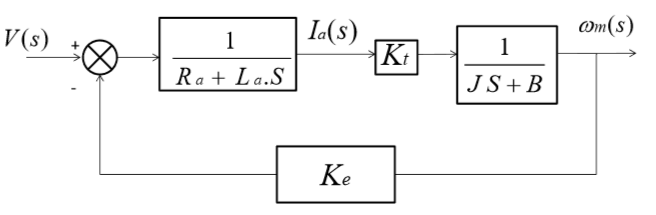
\includegraphics[scale= 0.55]{imagens/diagrama1_7.png}
\caption{\label{fig:D1_7} Modelo de segunda ordem do motor de corrente contínua.}
\caption*{Fonte: MARTINS, cap. 4, eslaide 2.}
\end{figure}


\subsubsection{Resposta da velocidade}

Considerando o diagrama de blocos da figura \ref{fig:D1_7} e  que:

$t \rightarrow \infty$;

$\omega_{m}(\infty) = \omega_{o}K$;

$\omega_{o} = \frac{V}{K_{e}}$;

$k = \frac{\tau_{b}}{\tau_{m}}$.

E os seguintes parâmetros:

$\tau_{b} = \frac{J}{B}$;

$\tau_{m} = \frac{R_{a}J}{K_{e}K_{t}}$;

$\tau_{a} = \frac{L_{a}}{R_{a}}$;

$\gamma_{3} = -\frac{C_{1}}{2} + \sqrt{\frac{C_{1}^{2}}{4} - C_{2}} $;

$\gamma_{4} = -\frac{C_{1}}{2} - \sqrt{\frac{C_{1}^{2}}{4} - C_{2}} $;

$C_{1} = \frac{1}{\tau_{a}} + \frac{1}{\tau_{b}}$

$C_{2} = \frac{1}{\tau_{a}\tau_{b}} + \frac{1}{\tau_{a}\tau_{m}}$;

A equação que modela a resposta da velocidade pode ser representada pela expressão a seguir:
\[\omega_{m}(t) = \omega_{o}K\left[1 + \frac{\gamma_{4}}{\gamma_{3} - \gamma_{4}}e^{\gamma_{3}t} - \frac{\gamma_{3}}{\gamma_{3} - \gamma_{4}}e^{\gamma_{4}t}\right]\]

\subsubsection{Resposta da corrente}

Ainda de acordo com o diagrama de blocos da figura \ref{fig:D1_7}, as considerações do item 2.6.1 e que:

$I_{SC} = \frac{V}{R_{a}}$

Para $t \rightarrow \infty \Rightarrow i_{a}(t) \rightarrow I_{SC}(1 - K)$

A função que expressa a resposta da corrente pode ser dada por:

\[i_{a}(t) = I_{SC}\left[1 - K + \frac{\frac{1}{\tau_{a}} + \gamma_{4} - \gamma_{4}K}{\gamma_{3} - \gamma_{4}}e^{\gamma_{3}t} - \frac{\frac{1}{\tau_{a}} + \gamma_{3} - \gamma_{3}K}{\gamma_{3} - \gamma_{4}}e^{\gamma_{4}t}\right]\]

Finalmente, as formas de onda da corrente e da velocidade para o modelo em questão são ilustradas na figura \ref{fig:G1_72}.

\begin{figure}[ht!]
\center
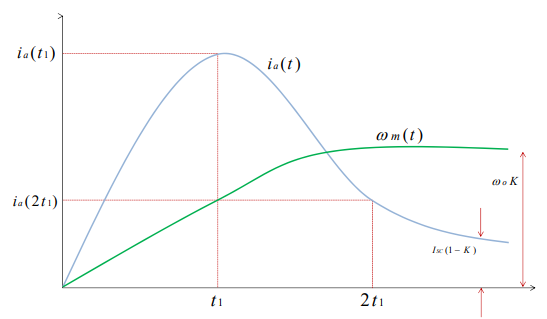
\includegraphics[scale= 0.55]{imagens/grafico1_72.png}
\caption{\label{fig:G1_72} Formas de onda da corrente e da velocidade no motor CC (Regime transitório e permanente) .}
\caption*{Fonte: MARTINS, cap. 4, eslaide 5.}
\end{figure}

Fazendo $\frac{\delta{i_{a}(t_{1}}}{\delta{t}} = 0$, obtém-se o ponto onde a corresnte é máxima.

Dessa forma:
\[ e^{\frac{t_{1}}{\tau_{a}}\left(\tau_{a}\gamma_{3} - \tau_{a}\gamma_{4}\right)} = \frac{\tau_{a}\gamma_{4}\left(1 + \tau_{a}\gamma_{3} - \tau_{a}\gamma_{3}K\right)}{\tau_{a}\gamma_{3}\left(1 + \tau_{a}\gamma_{4} - \tau_{a}\gamma_{4}K\right)}\]

\subsubsection{Medição dos parâmetros}

Para medir os parâmetros do motor de corrente contínua são empregados os seguintes métodos:

\begin{enumerate}
   \item Levantar as curvas $\omega_{m}(t)$ e i(t) experimentalmente. E a patir delas estabelecer as grandezas.
   
   $t_{1}, i_{t_{1}}, i_{2t_{1}}, I_{SC}(1-K), \omega_{o}K $
   
   \item Seja a relação de Pasek:
   
   \[\frac{i_{2t_{1}}}{i_{t_{1}}} = \frac{i_{t_{1}}}{I_{SC}}\]
   
   Desta forma pode-se determinar $I_{SC}$.
   
   \item Com a relação de $I_{SC}(1-K)$ determina-se o valor de K.
   
   \item Com a relação $I_{SC} = \frac{V}{R_{a}}$ determina-se o valor de $R_{a}$ visto que V é uma variável conhecida a partir dos ensaios.
   
   \item Com a relação $\frac{i_{2t_{1}}}{i_{t_{1}}}$ e com K, encontra-se no ábaco da figura \ref{fig:G1_73} e determina-se o valor de $\frac{\tau_{a}}{\tau_{m}}$.
   
   \item Com $\frac{\tau_{a}}{\tau_{m}}$ e K entra-se no ábaco da figura \ref{fig:G2_73} e determina-se $\frac{t_{1}}{\tau_{a}}$. Como $t_{1}$ é conhecido pode-se encontrar  $\tau_{a}$.
   
   \item Com a relação $\tau_{a} = \frac{L_{a}}{R_{a}}$ determina-se o valor de $L_{a}$.
   
   \item Com o valor de $\omega_{o}K$ e K, $\omega_{o}$ fica determinado.
   
   \item Com a relação de $\omega_{o} = V/K_{e}$, $k_{e}$ e $k_{t}$ ficam determinados.
   
   \item Com a relação $\tau_{a}/\tau_{m}$, $\tau_{m}$ pode ser determinado.
   
   \item Com a relação $\tau_{m} = \frac{R_{a}J}{K_{e}K_{t}}$, o valor de J fica determinado.
   
   \item Com a relação $K = \frac{\tau_{b}}{\tau_{b} + \tau_{m}}$, o valor de $\tau_{b}$ pode ser determinado.
   
   \item Com a relação $\tau_{b} = \frac{J}{B}$, o valor da constante de atrito B é determinado.
   

\end{enumerate}

\begin{figure}[ht!]
\center
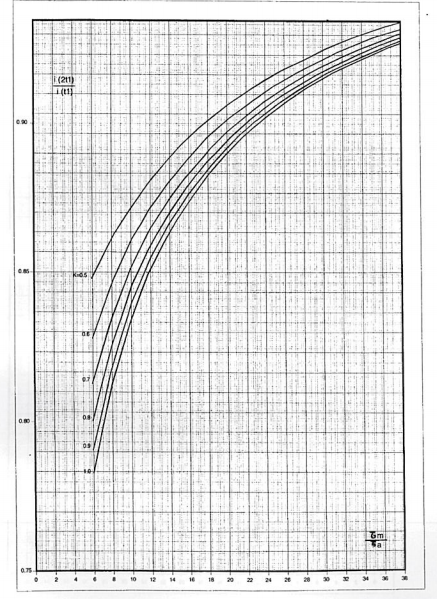
\includegraphics[scale= 0.55]{imagens/grafico1_73.png}
\caption{\label{fig:G1_73} Gráfico relacionando $i(2t_{1})/i(t_{1})$ em função de $\tau_{m}/\tau_{a}$ tendo K como parâmetro.}
\caption*{Fonte: Princípios de acionamento elétrico em corrente contínua (2006).}
\end{figure}

\begin{figure}[ht!]
\center
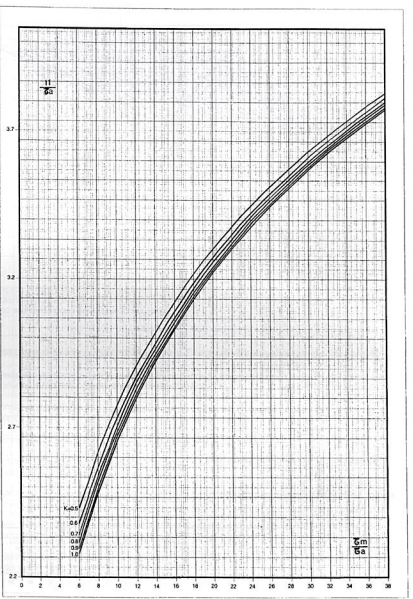
\includegraphics[scale= 0.55]{imagens/grafico2_73.png}
\caption{\label{fig:G2_73} Gráfico relacionando $t_{1}/\tau_{a}$ em função de $\tau_{m}/\tau_{a}$ tendo K como parâmetro.}
\caption*{Fonte: Princípios de acionamento elétrico em corrente contínua (2006) .}
\end{figure}

Os tópicos a seguir referem-se ao estudo da associação dos motores de corrente contínua aos conversores estáticos.



\subsection{Desempenho}

O motor de corrente contínua permite o controle da velocidade, pois é mais fácil de acionar em relação à maquinas de corrente alternada. O uso de conversores estáticos a tiristor ou transistor é a melhor solução para a variação da velocidade.

Portanto, devido a variedade de estruturas disponíveis, é necessário o uso de critérios para estabelecer qual a melhor solução para cada caso. Os critérios mais importantes são:

\begin{enumerate}
    \item Característica torque-velocidade: A presença de um conversor modifica a característica torque-velocidade natural do motor, é preciso então que as novas características sejam adequadas para a carga que se deseja acionar.
    
    \item Fator de potência: Estruturas e modos diferentes de controlá-las podem provocar consumos de reativos diferentes para uma mesma carga e uma mesma máquina. O fator de potência é dado por:
    \begin{equation*}
        FP = \frac{Potencia de entrada}{Volt.Amperes de entrada} = \frac{V.I_{1}.\cos{\phi_{1}}}{V.I}
    \end{equation*}
    
    onde:
    
    $I_{1} \rightarrow$ Valor eficaz da corrente fundamental.
    
    $I \rightarrow$ Valor eficaz da corrente total.
    
    $\phi_{1}  \rightarrow$  Ângulo entre a tensão e a corrente fundamental.
    
    \item Conteúdo Harmônico: É definido pela expressão a seguir:
    \[I_{h} = \frac{\sqrt{I^{2} - I_{1}^{2}}}{I_{1}}\]
    
    Quanto maior o conteúdo harmônico introduzido na rede, mais indesejável é o sistema conversor-motor CC.
    
    \item Fator de forma da corrente de armadura: O fator de forma é definido por:
    \begin{equation*}
        FF = \frac{I_{a_{eficaz}}}{I_{a_{medio}}}
    \end{equation*}
    
    $I_{a}$ é a corrente de armadura do motor.
    
    Quanto maior o fator de forma, maior será as perdas do motor. A corrente máxima do motor sempre deve ser respeitada.
    
    \item Corrente de pico: Quanto maior a corrente de pico, para uma corrente média, pior será o funcionamento do comutador do motor. A corrente máxima do motor sempre deve ser respeitada.
    
    \item Rendimento: Diferentes estruturas de comando podem propiciar rendimentos diferentes, para um dado motor e para uma dada carga.
\end{enumerate}


 
\subsection{Retificadores com carga RLE}

Um motor de corrente contínua com velocidade constante pode ser representados pela figura \ref{fig:C1-21-II}.

\begin{figure}[ht!]
\center
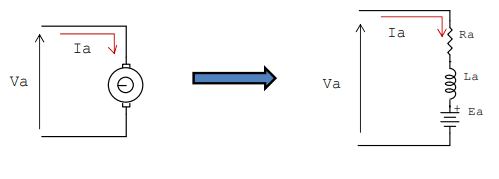
\includegraphics[scale= 0.88]{imagens/circuito1_21_II.png}
\caption{\label{fig:C1-21-II}Representação do motor CC com velocidade constante.}
\caption*{Fonte: MARTINS, cap. 5, eslaide 5.}
\end{figure}

Onde:

$R_{a} \rightarrow$ resistência de armadura.

$L_{a} \rightarrow$ indutância  de armadura.

$E_{a} = K_{a}\omega_{m} \rightarrow$ força contra-eletromotriz

Desta forma a figura \ref{fig:C2-21-II} representa um motor associado a um retificador controlado.

\begin{figure}[ht!]
\center
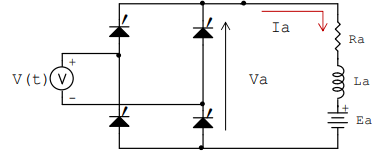
\includegraphics[scale= 0.88]{imagens/circuito2_21_II.png}
\caption{\label{fig:C2-21-II} Retificador controlado alimentando um motor CC operando com velocidade constante.}
\caption*{Fonte: MARTINS, cap. 5, eslaide 5.}
\end{figure}

Vale destacar que no acionamento dos motores CC considera-se os efeitos da condução descontínua.

\subsubsection{Ábaco de Pushlowski}
A figura \ref{fig:C1-22-II} representa a estrutura básica.

\begin{figure}[ht!]
\center
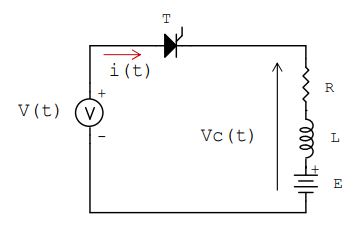
\includegraphics[scale= 0.88]{imagens/circuito1_22_II.png}
\caption{\label{fig:C1-22-II} Retificador monofásico controlado de meia-onda.}
\caption*{Fonte: MARTINS, cap. 6, eslaide 6.}
\end{figure}

E as formas de onda são (figura \ref{fig:G1-22-II}).

\begin{figure}[ht!]
\center
\includegraphics[scale= 0.88]{imagens/grafico1_22_II.png}
\caption{\label{fig:G1-22-II} Principais formas de onda.}
\caption*{Fonte: MARTINS, cap. 5, eslaide 6.}
\end{figure}

Onde:

$\alpha \rightarrow$ ângulo de disparo do tiristor.

$\beta \rightarrow$ ângulo de extinção do tiristor.

$\gamma = \beta - \alpha \rightarrow$ ângulo de condução.

\[v(t) = \sqrt{2}V\sin{\omega_{t}}\]

Onde V é o valor eficaz da tensão de entrada v(t).

Quando o tiristor conduz, no intervalo $(\alpha,\beta)$, a corrente é determinada pela seguinte equação:
\[v(t) = Ri(t) + L\frac{di(t)}{dt} + E\]

A solução dessa equação é dada por:

\[i(t) = \frac{\sqrt{2}V}{R}\left[\cos{\theta}\sin({\omega{t} - \theta}) - a + \left[a - \cos{\theta}\sin({\alpha - \theta})\right]e ^{-\frac{(\omega{t} - \alpha)}{\tan{\theta}}}\right]\]

\[a = \frac{E}{\sqrt{2}V}\]
\[\theta = \tan^{-1}{\frac{\omega{L}}{R}}\]

É importante salienta que o parâmetro "$a$" é proporcional a velocidade do motor CC $\rightarrow$ coeficiente de velocidade do sistema Retificador-Motor.

E, para $\omega{t} = \beta \Rightarrow i(t) = 0$. Portanto:

\[\left[\cos{\theta}\sin({\beta - \theta}) - a + \left[a - \cos{\theta}\sin({\alpha - \theta})\right]e ^{-\frac{(\beta - \alpha)}{\tan{\theta}}}\right] = 0\]

Nenhuma das variáveis da equação anterior podem ser explicitadas, portanto, utiliza-se o ábaco de Puschlowski (figura \ref{fig:A-22-II} que representa essa mesma equação para todos os retificadores a tiristor. Essa mesma expressão também pode ser solucionada numericamente.


\begin{figure}[ht!]
\center
\includegraphics[scale= 0.88]{imagens/abaco_22_II.png}
\caption{\label{fig:A-22-II} Ábaco de Puschlowski.}
\caption*{Fonte: MARTINS, cap. 5, eslaide 8.}
\end{figure}


A condução torna-se crítica quando:

\[ \gamma_{c} = \frac{2\pi}{p}\]

Onde:

$\gamma_{c} \rightarrow$ ângulo de condução crítica.

$p \rightarrow$ número de pulsos do retificador.

Como: $\gamma_{c} = \beta_{c} - \alpha_{c} \Rightarrow \alpha_{c} = \beta_{c} - \frac{2\pi}{p}$

No ábaco da figura \ref{fig:A-22-II} obtém-se o valor de $\cos{\theta}$ e $\theta$. E, com a relação $\tan{\theta} = \frac{\omega{L}}{R}$, determina-se o valor da indutância crítica $L_{c}$.

Com $L_{c} = L_{ext} + L$, é possível determinar a indutância externa para manter a condução contínua.

\subsubsection{Estruturas dos retificadores em questão}

\begin{figure}[ht!]
\center
\includegraphics[scale= 0.88]{imagens/tabela1_24_II.png}
\caption{\label{fig:T-24-II} Estruturas retificadoras.}
\caption*{Fonte: MARTINS, cap. 5, eslaide 11.}
\end{figure}

\subsubsection{Cálculo das tensões médias}

A tensão média produzida pelo retificador é dada pela seguinte expressão:
\[E_{dc} = \frac{1}{2\pi}{p} \int_{\alpha}^{\beta}\left(\sqrt{2}V\sin{\omega{t}}\right)d\omega{t}\]

Ou seja,
\[E_{dc} = \frac{\sqrt{2}}{2}\frac{p.V}{\pi}\left(\cos{\alpha} \cos{\beta}\right)\]

Quando a condução é contínua obtém-se:

\[\beta = \alpha + \frac{2\pi}{p}\]

Logo:

\[E_{dc} = \frac{p.V}{\sqrt{2}\pi}\left[\cos{\alpha} - \cos{\left(\alpha + \frac{2\pi}{p}\right)}\right]\]

A tensão média nos terminais da máquina é dada por:

\[E_{dc}' = RI_{dc} + E \]
\[RI_{dc} = E_{dc}' - E = \frac{p}{2\pi}\int_{\alpha}^{\beta}\left(\sqrt{2}V\sin{\omega{t} - E}\right)d\omega{t} \]

Portanto:

\[E_{dc}' = \frac{pV}{\sqrt{2}\pi}\left[\cos{\alpha} - \cos{\beta} - \frac{E}{\sqrt{2}V}\frac{2\pi}{p}\right]\]

Quando a condução é contínua $E_{dc}' = E_{dc}$.

\subsubsection{Expressão clássica da tensão}
Representa-se um ângulo de disparo $\psi$ definido de acordo com o número de pulsos do retificador. Assim, conforme a figura \ref{fig:G1-252-II}, tem-se:
\[Z = \frac{p\pi - 2\pi}{2p}\]

\begin{figure}[ht!]
\center
\includegraphics[scale= 0.88]{imagens/grafico1_252_II.png}
\caption{\label{fig:G1-252-II} Forma de onda da tensão oriunda de um retificador trifásico}
\caption*{Fonte: MARTINS, cap. 5, eslaide 15.}
\end{figure}

Deste modo,

\[Z + \psi = \alpha \Rightarrow \psi = \alpha - \frac{p\pi - 2\pi}{2\pi}\]

Portanto:

\[E_{dc} = \frac{p.V}{\pi.\sqrt{2}}\left[\cos\left(\psi + \frac{\pi.p - 2\pi}{2p}\right) - \cos\left(\psi + \frac{\pi}{2} - \frac{\pi}{p} + \frac{2\pi}{p}\right)\right]\]

\[E_{dc} = \frac{\sqrt{2}.p.V}{\pi}\left[\sin\left(\frac{\pi}{p}\right)\cos{(\psi)}\right]\]

Essa última é a expressão clássica para os retificadores , válida somente para condução contínua e p>1.

Para $\frac{\pi}{2} < \psi < \pi  \Rightarrow E_{dc} < 0$

Isso significa que o conversor funciona como inversor não autônomo; e a máquina pode fornecer energia á rede nessa condição. 

\subsubsection{Excitação separada e retificador a tiristor (caso geral)}

Parte-se da estrutura conforme na figura \ref{fig:C1-26-II}.

\begin{figure}[ht!]
\center
\includegraphics[scale= 0.88]{imagens/grafico1_26_II.png}
\caption{\label{fig:C1-26-II} Motor CC alimentado por retificador a tiristor}
\caption*{Fonte: MARTINS, cap. 5, eslaide 16.}
\end{figure}

Conhecendo-se os parâmetros do motor, deseja-se determinar a sua característica torque-velocidade quando associado ao retificador. Portanto foi estabelecido que para a condução descontínua:

\[\frac{RI_{dc}}{\sqrt{2}V} = \frac{p}{2\pi}\left[\cos\alpha - \cos\beta - a(\beta - \alpha)\right]\]

E, para condução contínua,

\[\frac{RI_{dc}}{\sqrt{2}V} = \frac{p}{2\pi}\left[\cos\alpha - \cos\left(\alpha + \frac{2\pi}{p}\right) - a\frac{2\pi}{p}\right]\]

Para um $I_{f}$ constante $\Rightarrow T = f(I_{dc})$. Ou seja, o torque é proporcional a $I_{dc}$. Portanto:
\[\frac{R}I_{dc}{V\sqrt{2}} = t_{f}\]

$t_{f}$ é o fator de torque.

Desse modo obtém-se:

$t_{f} = \frac{p}{2\pi}\left[\cos{\alpha} - \cos{\beta} \alpha\left(\beta - \alpha\right)\right] \rightarrow$ para condução contínua.

$t_{f} = \frac{p}{2\pi}\left[\cos{\alpha} - \cos\left(\alpha + \frac{2\pi}{p}\right) - a.\frac{2\pi}{p} \right] \rightarrow$ para condução descontínua.

Sendo assim, pode-se obter um conjunto de características $t_{f} = f(a)$, onde p é fixado e $\alpha$ é considerado um parâmetro. 

Para condução contínua, utiliza-se a primeira definição de $t_{f}$. E, quando a condução é descontínua, para um dado $\alpha$ deve-se calcula $\beta$ a partir do ábaco de Pushlowski, para em seguida determinar $t_{f}$


 
\subsection{Excitação separada e retificador controlado}

Estudaremos agora o motor CC com excitação separada alimentado por um retificador controlado.

\subsubsection{Retificador controlado de meia onda}

As figuras \ref{fig:C1-31-II} e \ref{fig:G1-31-II} representam respectivamente o circuito e as formas de onda do retificador controlado de meia onda.
 
 \begin{figure}[ht!]
\center
\includegraphics[scale= 0.88]{imagens/circuito1_31_II.png}
\caption{\label{fig:C1-31-II}Retificador controlado de meia onda}
\caption*{Fonte: MARTINS, cap. 6, eslaide 2.}
\end{figure}

\begin{figure}[ht!]
\center
\includegraphics[scale= 0.88]{imagens/grafico1_31_II.png}
\caption{\label{fig:G1-31-II}Principais formas de onda}
\caption*{Fonte: MARTINS, cap. 6, eslaide 3.}
\end{figure}

Onde:

$V_{m}(t) \rightarrow$ tensão nos terminais da máquina.

$i(t) \rightarrow$ corrente de armadura.

$E_{a} \rightarrow$ força eletromotriz da máquina.

$v(t) \rightarrow$ tensão de alimentação.

Considerando $\omega_{m}$ constante, $E_{a}$ também será constante. A velocidade sofre uma pequena ondulação, pois o torque elétrico produzido pelo motor é pulsado. 

A tensão média nos terminais da máquina pode ser obtida a partir da seguinte expressão:
\[V_{m} = R.I_{a} + E_{a}\]
\[R.I_{a} = \frac{\sqrt{2}.V}{2\pi}\left[\cos{\alpha} - \cos{\beta} - \frac{E_{a}}{\sqrt{2}V}\left(\beta - \alpha\right)\right]\]

Logo, a expressão da característica torque velocidade é dada por:
\[\frac{R.I_{a}}{\sqrt{2}V}  = \frac{I}{2\pi}\left[\cos{\alpha} - \cos{\beta} - \frac{E_{a}}{\sqrt{2}V}\left(\beta - \alpha\right)\right]\]

Onde:

\[\frac{R.I_{a}}{\sqrt{2}V} = t_{f}\]
\[\frac{E_{a}}{\sqrt{2}V} = a\]

Para $I_{f}$ constante o torque é proporcional a $I_{a}$. Logo, $t_{f}$ é definido como fator de torque. Portanto:

\[t_{f} = \frac{1}{2\pi}\left[\cos{\alpha} - \cos{\beta} - a\left(\beta - \alpha\right)\right]\]

A expressão anterior define as características torque-velocidade do motor associado ao retificador. Assim tem-se a seguinte função: $t_{f} = f(a)$, onde $\beta$ é fixado, e $\alpha$ é um parâmetro.

\subsection{Retificador de meia onda com diodo de roda livre}

O emprego do diodo de roda livre aprimora o comportamento do motor. Sua estrutura está representada na figura \ref{fig:C1-32-II}

\begin{figure}[ht!]
\center
\includegraphics[scale= 0.88]{imagens/circuito1_32_II.png}
\caption{\label{fig:C1-32-II} Retificador de meia onda com roda livre}
\caption*{Fonte: MARTINS, cap. 6, eslaide 6.}
\end{figure}

E as formas de onda estão ilustradas na fig \ref{fig:C1-32-III}

\begin{figure}[ht!]
\center
\includegraphics[scale= 0.88]{imagens/circuito1_32_II.png}
\caption{\label{fig:C1-32-III} Principais formas de onda}
\caption*{Fonte: MARTINS, cap. 6, eslaide 6.}
\end{figure}

Neste caso:

\[i_{1} = \frac{\sqrt{2}V}{R}\left\{\cos{\theta}\sin\left(\omega{t} - \theta\right) - a + \left[a - \cos{\theta}\sin{\left(\alpha - \theta\right)}\right]e^{-\left(\omega{t} - \alpha\right)/\tan{\theta}}\right\}\]

\[i_{2}(t) = i_{1}(\pi)e^{-\frac{\omega{t}}{\tan{\theta}}} - \frac{E_{a}}{R}\left(1 - e^{-\frac{\omega{t}}{\tan{\theta}}}\right)\]

Quando $\omega{t} = \beta \Rightarrow i_{2}(t) = 0$. Assim, levando essa conclusão nas equações anteriores tem-se que:
\[\beta = \tan{\theta}.ln\left[\frac{R.i_{1}(\pi)}{E_{a}} + 1\right]\]

O valor da tensão média nos terminais do motor é dado abaixo:

\[V_{m} = E_{a} - \frac{(\beta - \alpha)}{2\pi}E_{a} + \frac{\sqrt{2}V}{2\pi}\left(1 + \cos{\alpha}\right)\]

Onde:
\[V_{m} = R.I_{a} + E_{a} \Rightarrow R.I_{a} = V_{m} - E_{a}\]

Logo,
\[R.I_{a} = \frac{\sqrt{2}V}{2\pi}\left[1 + \cos{\alpha} - \frac{E_{a}}{\sqrt{2}V}\left(\beta - \alpha\right)\right]\]

Definindo $t_{f} = \frac{R.I_{a}}{\sqrt{2}V} \rightarrow$ fator torque, obtém-se:

\[t_{f} = \frac{1}{2\pi}\left[1 + \cos{\alpha} - a\left(\beta - \alpha\right)\right]\]

A partir desta equação é possível determinar a característica torque-velocidade do motor CC.

\subsection{Retificador misto de onda completa com diodo de roda livre}

A estrutura de potência do retificador misto de onda completa com diodo de roda livre alimentando o motor CC é apresentado na figura \ref{fig:C1-33-II}

\begin{figure}[ht!]
\center
\includegraphics[scale= 0.88]{imagens/circuito1_33_II.png}
\caption{\label{fig:C1-33-II} Retificador misto de onda completa com diodo de roda livre}
\caption*{Fonte: MARTINS, cap. 6, eslaide ARRUMAR.}
\end{figure}

Esta estrutura é uma das mais empregadas industrialmente para motores CC até 10 KW. É econômica por conter somente dois tiristores. A presença do diodo $D_{RL}$, aliada à retificação de onda completa contribui para a redução das harmônicas de corrente de armadura e para minimizar os problemas ligados à condução descontínua. As de formas de onda, para condução descontínua e contínua, são apresentadas nas figuras \ref{fig:G1-33-II} e \ref{fig:G2-33-II}

\begin{figure}[ht!]
\center
\includegraphics[scale= 0.88]{imagens/grafico1_33_II.png}
\caption{\label{fig:G1-33-II} Principais formas de onda para condução contínua}
\caption*{Fonte: MARTINS, cap. 6, eslaide ARRUMAR.}
\end{figure}

\begin{figure}[ht!]
\center
\includegraphics[scale= 0.88]{imagens/grafico2_33_II.png}
\caption{\label{fig:G2-33-II} Principais formas de onda para condução descontínua}
\caption*{Fonte: MARTINS, cap. 6, eslaide ARRUMAR.}
\end{figure}

Quando o tiristor conduz, a tensão nos terminais do motor é igual a tensão da rede. Durante a roda livre a tensão é nula, e durante a descontinuidade a tensão nos terminais da máquina é a própria força contra eletromotriz do motor.


\subsubsection{Equacionamento básico}

\[i_{1} = \frac{\sqrt{2}V}{R}\left\{\cos{\theta}\sin\left(\omega{t} - \theta\right) - a + \left[a - \cos{\theta}\sin{\left(\alpha - \theta\right)}\right]e^{-\left(\omega{t} - \alpha\right)/\tan{\theta}}\right\}\]

\[i_{2}(t) = i_{1}(\pi)e^{-\frac{\omega{t}}{\tan{\theta}}} - \frac{E_{a}}{R}\left(1 - e^{-\frac{\omega{t}}{\tan{\theta}}}\right)\]

\[\beta = \tan{\theta}.ln\left[\frac{F_{1}(\theta,a,\alpha,\pi)}{a} + 1\right]\]

Sendo $F_{1}(\theta,a,\alpha,\pi) = \cos{\theta}\sin\left(\pi - \theta\right) - a + \left[a - \cos{\theta}\sin{\left(\alpha - \theta\right)}\right]e^{-\left(\pi - \alpha\right)/\tan{\theta}} $.

Deseja-se, estabelecer as características torque-velocidade do motor. Assim:

\begin{itemize}
    \item Condução descontínua:
    
	\[t_{f} = \frac{1}{\pi}\left[1 + \cos{\alpha} - a(\beta - \alpha)\right]\]
    
    \item Condução contínua:
    
	\[t_{f} = \frac{1}{\pi}\left[1 + \cos{\alpha} - \pi{a}\right]\]
    
    
\end{itemize}

\subsubsection{Cálculo da indutância crítica}

A condução é crítica quando $\beta = \pi + \alpha$. Portanto, a partir da seguinte expressão:

\[\beta = \tan{\theta}.ln\left[\frac{F_{1}(\theta,a,\alpha,\pi)}{a} + 1\right]\]

Obtém-se:

\[\pi + \alpha = \tan{\theta}.ln\left[\frac{F_{1}(\theta,a,\alpha,\pi)}{a} + 1\right]\]

Logo, sabendo a e $\alpha$, pode-se determinar $\theta$; e consequentemente pode-se determinar a indutância crítica:

\[\tan{\theta_{c}} = \frac{\omega.L_{c}}{R}\]
\[L_{c} = \frac{R}{\omega}\tan{\theta_{c}}\]


 
\subsection{Conversores CC-CC}

O uso de conversores CC-CC é indicado quando deseja-se controlar um motor CC. A figura \ref{fig:C1-41-II} representa a estrutura básico desse conversor.

\begin{figure}[ht!]
\center
\includegraphics[scale= 0.88]{imagens/circuito1_41_II.png}
\caption{\label{fig:C1-41-II} Motor CC acionado por conversores CC-CC}
\caption*{Fonte: MARTINS, cap. 7, eslaide ARRUMAR.}
\end{figure}

Mesmo quando a fonte é de corrente alternada, o emprego dos conversores CC-CC pode ser muito interessante pois, em relação aos retificadores controlados, os conversores CC-CC operam com maior frequência, podendo assim obter condução contínua sem o emprego de filtros volumosos e a resposta torna-se mais rápida. 




\FloatBarrier
\newpage

\section{Máquinas de Corrente Alternada Assíncronas}


Uma máquina de corrente contínua pode funcionar tanto como um gerador, convertendo energia mecânica em energia elétrica, quanto como um motor, convertendo energia elétrica em mecânica. Apesar de a energia elétrica ser comumente distribuída (no nível do consumidor) em corrente alternada, os motores de corrente contínua possuem grande participação na indústrias, uma vez que permitem facilmente a variação de velocidade, por exemplo, de uma esteira ou um comboio. 

Por outro lado, componentes eletrônicos de tensão alternada, cada vez mais acessíveis, são capazes de controlar a velocidade de motores assíncronos da mesma forma, logo, pelo seu melhor custo benefício, eles vêm substituindo os motores de corrente contínua na maior parte das aplicações. De toda forma, o estudo dos motores de corrente contínua é fundamental pois introduz os conceitos básicos do funcionamento de máquinas elétricas. A figura \ref{fig:MCC} mostra esquematicamente uma máquina de corrente contínua elementar.

\begin{figure}[ht!]
\center
\includegraphics[scale=0.66]{imagens/maquina_cc.png}
\caption{\label{fig:MCC}Máquina de corrente contínua elementar.}
\caption*{Fonte: Máquinas de corrente contínua \protect\footnotemark}
\end{figure}

\footnotetext{Disponível em: <http://www.gsep.ene.unb.br/osem/ivan/Conversao> Acesso em out. 2018.}



\subsection{Aspectos construtivos}

Os principais componentes das máquinas de corrente alternada assíncronas estão o rotor e o estator. O rotor, por definição, é a peça que gira em torno do seu próprio eixo. A máquina de indução, ao contrário da máquina CC, possui um entreferro uniforme. O rotor pode ser do tipo gaiola de esquilo ou do tipo bobinado.
    
Os enrolamentos do estator aa’, bb’ e cc’ estão defasados de 120 graus entre si. Quando uma corrente alternada passa por um enrolamento ela produz uma força magneto-motriz também alternada e centrada no eixo do enrolamento. Cada força magneto-motriz é representada por um vetor com magnitude proporcional ao valor instantâneo da corrente. As correntes instantâneas em cada enrolamento são mostradas na figura \ref{fig:11}.

\begin{figure}[hbt]
    \center 
    \includegraphics[scale=1.2]{imagens/11.PNG}
    \caption{Correntes instantâneas em cada enrolamento.}\label{fig:11}
\end{figure}

A força magneto-motriz resultante é composta pelas três componentes de força
magneto-motriz, que pode ser visualizada graficamente como na figura \ref{fig:12}.

\begin{figure}[ht]
    \center 
    \includegraphics[scale=1.2]{imagens/12.PNG}
    \caption{Campo magnético girante.}\label{fig:12}
\end{figure}

No instante de tempo $t_o$, a corrente na fase a passa por um máximo positivo e as correntes nas fases b e c por metade da amplitude máxima negativa. Devido ao fato da corrente na fase a estar em um instante de máximo, a força magneto-motriz produzida por este enrolamento é máxima.

A força magneto-motriz, resultante da composição vetorial das forças magneto-motriz devido aos três enrolamentos, é dada pela equação
$$\vec{F} = \frac{2}{3}.F_{max}$$

A força magneto-motriz resultante é distribuída senoidalmente ao longo do entreferro. Analisando o que acontece à medida que as correntes em cada enrolamento variam senoidalmente, nota-se que o vetor resultante F possui a mesma amplitude em todos os
instantes de tempo, mas ele gira em sentido anti-horário.



\subsection{Princípio de funcionamento}

O funcionamento da máquina assíncrona pode ser representado utilizando um ímã permanente e um disco livre para girar, como mostrado na figura \ref{fig:13}.

\begin{figure}[ht!]
\center 
\includegraphics[scale=1.2]{imagens/13.PNG}
\caption{Princípio de funcionamento da máquina assíncrona.}\label{fig:13}
\end{figure}

O ímã permanente é suspenso sobre um disco metálico. O fluxo magnético produzido pelo ímã permanente flui através do circuito magnético composto pelo ímã permanente, os entreferros e a placa de ferro. Ao girar o ímã permanente, o disco que se encontra sob o ímã também gira. O disco acompanha o movimento de rotação do ímã permanente devido à circulação de correntes induzidas. Estas correntes são induzidas devido ao movimento relativo entre o disco e o ímã permanente. As correntes induzidas tendem a produzir, de acordo com a lei de Lenz, um polo sul magnético no disco sob o polo norte magnético girante do ímã permanente, assim como um polo norte magnético no disco sob o polo sul magnético girante do ímã permanente. Enquanto o ímã continua seu movimento em relação ao disco, continuará a indução de correntes parasitas e polos magnéticos com polaridades opostas. O disco, desta forma, gira no mesmo sentido que o ímã permanente, mas deve girar a uma velocidade menor para que haja uma velocidade relativa entre o ímã permanente e o disco metálico.



\subsection{Tensões induzidas}

Quando correntes balanceadas circulam pelos enrolamentos trifásicos do estator, um campo magnético senoidal distribuído gira no entreferro da máquina. O efeito produzido por este campo é similar ao produzido por um par de polos girando no entreferro, de tal forma que a distribuição de densidade de fluxo ao longo deste entreferro seja senoidal com o pico ao longo do eixo dos polos magnéticos.

\begin{figure}[ht!]
\center 
\includegraphics[scale=1.2]{imagens/14.PNG}
\caption{Distribuição de densidade de fluxo ao longo do entreferro.}\label{fig:14}
\end{figure}

A densidade do fluxo ao longo do entreferro é representado por:

$$B(\theta) = B_{max}. \cos(\theta)$$

A força eletromotriz, que é dada pela variação do fluxo no tempo multiplicada pelo número de espiras, permite escrever a expressão.

$$e_a = \omega . N. {\phi}_p . K_w = E_{max} . \sin(\omega t)$$

A tensão eficaz por fase:

$$E_1 = 4,44 . f_1 . N_1 . \phi_p . K_w$$

Com o fator de enrolamento $K_w$ variando de 0,85 à 0,95.



\subsection{Escorregamento}

Quando o enrolamento do estator for conectado a uma fonte de alimentação trifásica e o circuito do rotor é fechado, as correntes induzidas no rotor irão produzir um campo magnético que irá interagir com o campo magnético girante no entreferro, dando origem a um torque. O rotor, se livre, irá iniciar o movimento de rotação. De acordo com a lei de Lenz, o rotor gira na direção do campo magnético girante de tal maneira que a velocidade relativa entre o campo magnético girante e o enrolamento do rotor diminua. O rotor irá atingir uma velocidade de rotação n que é inferior à velocidade de rotação síncrona. A diferença entre a velocidade síncrona do campo magnético girante e a velocidade do rotor é denominada escorregamento e é definida através da equação:

$$S = \frac{n_s - n}{n_s}$$

A frequência da corrente induzida no circuito do rotor é dada pela expressão:

$$f_2 = s  f_1$$



\subsection{Circuito equivalente}

O circuito equivalente pode ser utilizado para estudar e antecipar o desempenho da máquina de indução trifásica com apreciável proximidade do seu comportamento real. O circuito equivalente mostrado na figura abaixo considera as perdas por condução por fase no enrolamento de estator através  da resistência $R_1$, o fluxo de dispersão por fase no enrolamento de estator através da reatância $X_1$, as perdas no núcleo através da resistência $R_c$, a energia necessária para magnetização do núcleo através da reatância $X_m$, o fluxo de dispersão no rotor refletido ao estator através da reatância $X_2$’ e a resistência de condução do enrolamento do rotor refletido ao estator. Para se determinar os parâmetros do circuito elétrico equivalente podem-se utilizar os ensaios sem carga e com rotor bloqueado.

\begin{figure}[ht!]
\center 
\includegraphics[scale=1.2]{imagens/15.PNG}
\caption{Circuito elétrico equivalente para a máquina de indução.}
\end{figure}


\subsubsection{Alimentação com tensão senoidal, frequência variável em regime permanente}
O motor de indução em regime permanente com alimentação senoidal pode ser representado pelo seguinte circuito conforme na figura \ref{fig:fig1-1}.

\begin{figure}[ht!]
\center
\includegraphics[scale= 0.88]{imagens/fig1-1.PNG}
\caption{\label{fig:fig1-1}Modelo em regime permanente senoidal para o motor de indução.}
\caption*{Fonte: MARTINS, eslaide 01 Acionamentos elétricos - Cap VIII}
\end{figure}

Note que\\

$r_{1}$ = resistência ôhmica do estator por fase;\\
$x_{1}$ = reatância de dispersão do estator por fase;\\
$r_{s}$ = resistência ôhmica do rotor por fase;\\
$x_{2}$ = reatância de dispersão do rotor por fase;\\
$w_{r}$ = frequência de pulsação das correntes do rotor;\\
$w_{s}$ = frequência de pulsação das correntes do estator;\\
$S$ = escorregamento do motor;\\
$V_{l} = V_{S}$ = tensão estatória por fase;\\

Para o cálculo do torque eletromagnético emprega-se o circuito da figura \ref{fig:fig1-1sss}.

\begin{figure}[ht!]
\center
\includegraphics[scale= 0.88]{imagens/fig1-2.PNG}
\caption{\label{fig:fig1-1sss}Circuito equivalente para o cálculo do torque.}
\caption*{Fonte: MARTINS, eslaide 01 Acionamentos elétricos - Cap VIII}
\end{figure}

O torque eletromagnético é dado por:
\[T = \frac{1}{w_{sin}}\cdot \frac{q \cdot V_{1a}^2 \cdot \left ( \frac{r_{2}}{S} \right )}{\left [ \left ( R_{1} + \frac{r_{2}}{S}\right )^2 + \left ( X_{1}+x_{2} \right )^2\right ]}\]

Sabe-se que a velocidade de uma maquina síncrona é calculada sendo sessenta vezes a frequência do estator, dividido pelo numero de polos.
Além disso, sabe-se que a velocidade do rotor é aproximadamente igual a velocidade síncrona.
Assim, variando a frequência pode-se variar a velocidade da máquina. 
Por outro lado, o fluxo magnético é diretamente proporcional a tensão e inversamente a frequência. Logo, para variar a frequência deve-se variar a tensão.

O torque máximo desenvolvido pelo motor de indução, considerando impedância do estator desprezível é
\[T_{max} = k\cdot \phi_{S} ^2\]
O que mostra que o valor do torque máximo depende somente do fluxo no entreferro da maquina, não da frequência de operação.

Aproximando a frequência do estator com a frequência síncrona e fazendo algumas considerações obtém-se a equação do torque
\[T = \frac{p\cdot q}{r_{2}}\cdot \phi _S^2 \cdot w_{r}\]
O que demonstra que quando o fluxo é constante, com baixos valores de escorregamento, o torque é proporcional a pulsação rotórica.

A figura \ref{fig:fig1.3} ilustra as características torque/velocidade para um motor de indução com alimentação senoidal

\begin{figure}[ht!]
\center
\includegraphics[scale= 0.88]{imagens/fig1-3.PNG}
\caption{\label{fig:fig1.3}Motor de indução com alimentação senoidal a frequência variável.}
\caption*{Fonte: MARTINS, eslaide 01 Acionamentos elétricos - Cap VIII}
\end{figure}

É visto que o torque máximo não é preservado quando V/f é constante. Assim em acionamentos melhores, emprega-se outra lei de fluxo, mais precisa.

A figura \ref{fig:fig1.4} mostra o fluxo magnetizante quando V/f é constante.

\begin{figure}[ht!]
\center
\includegraphics[scale= 0.88]{imagens/fig1-4.PNG}
\caption{\label{fig:fig1.4}Fluxo magnetizante em função da frequência de alimentação do estator e da frequência do rotor.}
\caption*{Fonte: MARTINS, eslaide 01 Acionamentos elétricos - Cap VIII}
\end{figure}

A figura \ref{fig:fig1.5} mostra o torque máximo quando V/f é constante.

\begin{figure}[ht!]
\center
\includegraphics[scale= 0.88]{imagens/fig1-5.PNG}
\caption{\label{fig:fig1.5}Torque máximo em função da frequência de alimentação.}
\caption*{Fonte: MARTINS, eslaide 01 Acionamentos elétricos - Cap VIII}
\end{figure}

Observa-se que este método não pode ser empregado para cargas com altos torques em baixas velocidades.

Visto o modelo do motor de indução na forma complexa para alimentação senoidal em regime permanente, é estabelecida a lei V/f que permite manter o fluxo no entreferro constante.

\[\left | \bar{V_{s}} \right | = \frac{\left | \bar{\phi _{s}} \right | }{K_{s}}\cdot \sqrt{\frac{\left ( 1-w_{r}\cdot K_{r}\cdot w_{s}\cdot K_{s} \cdot \sigma\right )^2+\left ( w_{s}\cdot K_{s}+ w_{r}\cdot K_{r} \right )^2}{1+w_{r}^2\cdot K_{r}^2\cdot \sigma ^2}}\]

Assim, para que o fluxo se mantenha constante é necessário variar a tensão em função da frequência do estator e do rotor.
Simplificando a expressão através de considerações obtém-se:

\[\left( | \bar{V_{s}} \right) | = \left( | \bar{\phi _{s}} \right) \cdot w_{s}|\]

Que é a lei mais empregada devido a sua simplicidade.

\begin{figure}[ht!]
\center
\includegraphics[scale= 0.88]{imagens/fig1-6.PNG}
\caption{\label{fig:fig1.6}Lei V/f para $f_{r}=0$}
\caption*{Fonte: MARTINS, eslaide 02 Acionamentos elétricos - Cap IX}
\end{figure}

A lei de fluxo exata em regime permanente, obtida através da equação da lei V/f para fluxo constante e de alguns parâmetros é representada no gráfico da figura \label{fig:fig1.7}.

\begin{figure}[ht!]
\center
\includegraphics[scale= 0.88]{imagens/fig1-7.PNG}
\caption{\label{fig:fig1.7}Representação gráfica da lei de fluxo exata em regime permanente.}
\caption*{Fonte: MARTINS, eslaide 02 Acionamentos elétricos - Cap IX}
\end{figure}

A alimentação é direta, com fluxo constante, quando \[V_{s}/w_{s}\] é constante e \[w_{r}\] é variável.

\begin{figure}[ht!]
\center
\includegraphics[scale= 0.88]{imagens/fig1-8.PNG}
\caption{\label{fig:fig1.8}Torque versos velocidade pela lei de fluxo correta.}
\caption*{Fonte: MARTINS, eslaide 02 Acionamentos elétricos - Cap IX}
\end{figure}

\begin{figure}[ht!]
\center
\includegraphics[scale= 0.88]{imagens/fig1-9.PNG}
\caption{\label{fig:fig1.9}Representação em blocos da alimentação direta.}
\caption*{Fonte: MARTINS, eslaide 02 Acionamentos elétricos - Cap IX}
\end{figure}

São vistas as características torque-velocidade.

\begin{figure}[ht!]
\center
\includegraphics[scale= 0.88]{imagens/fig1-10.PNG}
\caption{\label{fig:fig1-10}Curva característica de torque-velocidade.}
\caption*{Fonte: MARTINS, eslaide 02 Acionamentos elétricos - Cap IX}
\end{figure}

A alimentação direta apresenta problemas fundamentais como a possibilidade de perda de estabilidade e possibilidade de haver solicitação excessiva de corrente do conversor.

\begin{figure}[ht!]
\center
\includegraphics[scale= 0.88]{imagens/fig1-11.PNG}
\caption{\label{fig:fig1-11} Curva característica de torque-velocidade.}
\caption*{Fonte: MARTINS, eslaide 02 Acionamentos elétricos - Cap IX}
\end{figure}

A corrente pode assumir valores elevados no inversor e danificar o equipamento.

\begin{figure}[ht!]
\center
\includegraphics[scale= 0.88]{imagens/fig1-12.PNG}
\caption{\label{fig:fig1-12}Curva característica de torque-velocidade.}
\caption*{Fonte: MARTINS, eslaide 02 Acionamentos elétricos - Cap IX}
\end{figure}

Quando a frequência é subitamente alterada, o torque de carga torna-se maior que o elétrico e o motor bloqueia.

Para evitar esses problemas a máquina é alimentada com frequência de rotor imposto (auto-pilotagem).

\begin{figure}[ht!]
\center
\includegraphics[scale= 0.88]{imagens/fig1-13.PNG}
\caption{\label{fig:fig1-13}Representação em blocos da auto-pilotagem.}
\caption*{Fonte: MARTINS, eslaide 02 Acionamentos elétricos - Cap IX}
\end{figure}

\begin{figure}[ht!]
\center
\includegraphics[scale= 0.88]{imagens/fig1-14.PNG}
\caption{\label{fig:fig1-14}Curva característica de torque-velocidade.}
\caption*{Fonte: MARTINS, eslaide 02 Acionamentos elétricos - Cap IX}
\end{figure}

A partir dos blocos da auto-pilotagem pode-se incluir um regulador de velocidade.

\begin{figure}[ht!]
\center
\includegraphics[scale= 0.88]{imagens/fig1-15.PNG}
\caption{\label{fig:fig1-15}Representação em blocos da auto-pilotagem com regulação de velocidade.}
\caption*{Fonte: MARTINS, eslaide 02 Acionamentos elétricos - Cap IX}
\end{figure}

Assim, agindo-se sobre o conversor causa-se uma variação na tensão E. Essa, por sua vez, é proporcional a frequência de funcionamento do inversor e com isso consegue-se manter a relação \[V_{s}/w_{s}\] constante.

\begin{figure}[ht!]
\center
\includegraphics[scale= 0.88]{imagens/fig1-16.PNG}
\caption{\label{fig:fig1-16}Representação em blocos do controle indireto do torque máximo.}
\caption*{Fonte: MARTINS, eslaide 02 Acionamentos elétricos - Cap IX}
\end{figure}

Através de análise obtém-se
\[I_{cc} \approx K_{s}w_{r},\]
logo, limitando-se a corrente, limita-se a velocidade.

\begin{figure}[ht!]
\center
\includegraphics[scale= 0.88]{imagens/fig1-17.PNG}
\caption{\label{fig:fig1-17}Representação em blocos do controle indireto do torque máximo com limitação da corrente $I_{cc}$.}
\caption*{Fonte: MARTINS, eslaide 02 Acionamentos elétricos - Cap IX}
\end{figure}

Ainda, é possível controlar indiretamente a frequência retórica utilizando-se outro princípio. Partindo da equação do torque, através de considerações obtém-se que
\[\bar{I}_{1max} =  \bar{I}_{2max} + \bar{I}_{m}.\]
Portanto, limitando-se $\bar{I}_{2max}$, consequentemente de $w_{r}$ e do torque.

\begin{figure}[ht!]
\center
\includegraphics[scale= 0.88]{imagens/fig1-18.PNG}
\caption{\label{fig:fig1-18}Representação em blocos da auto-pilotagem com regulação de velocidade.}
\caption*{Fonte: MARTINS, eslaide 02 Acionamentos elétricos - Cap IX}
\end{figure}

\subsubsection{Corrente do estator e torque para alimentação retangular em tensão}

Quando o motor de indução, conectado em Y é alimentado por um inversor do tipo 180o, a tensão em cada uma das fases possui forma como visível na figura \ref{fig:fig21}.

\begin{figure}[ht!]
\center
\includegraphics[scale= 0.88]{imagens/fig21.JPG}
\caption{\label{fig:fig21}Tensão aplicada a uma fase do estator.}
\caption*{Fonte: MARTINS, Acionamentos elétricos - Cap X.}
\end{figure}

A tensão de fase é
\[ v_{n}(t) = \frac{2E}{\pi }\cdot \frac{1}{n} \sin{nwt} \]

Os circuitos equivalentes são como na figura \ref{fig:fig22}.

\begin{figure}[ht!]
\center
\includegraphics[scale= 0.88]{imagens/fig22.JPG}
\caption{\label{fig:fig22}Circuitos elétricos equivalentes para as tensão fundamental e harmônica.}
\caption*{Fonte: MARTINS, Acionamentos elétricos - Cap X.}
\end{figure}

A partir desses circuitos obtém-se

\[ i(t) = \frac{2E}{\pi }\left [ \frac{1}{\left | Z_{1} \right |} \sin{(wt-\theta _{1})} + \sum_{n=5}^{\infty } \frac{1}{n^2(x_{1}+x_2)} \sin{\left ( nwt-\frac{\pi }{2} \right )} \right ] \]

Empregando-se o método das harmônicas obtém-se

\begin{figure}[ht!]
\center
\includegraphics[scale= 0.88]{imagens/fig23.JPG}
\caption{\label{fig:fig23}Comportamento da corrente do motor com escorregamento de 0,1.}
\caption*{Fonte: MARTINS, Acionamentos elétricos - Cap X.}
\end{figure}

\begin{figure}[ht!]
\center
\includegraphics[scale= 0.88]{imagens/fig24.JPG}
\caption{\label{fig:fig24} Comportamento da corrente do motor com escorregamento de 0,025.}
\caption*{Fonte: MARTINS, Acionamentos elétricos - Cap X.}
\end{figure}

De acordo com o modelo para o motor de indução, na forma complexa, com o referencial fixo no estator do motor, após as devidas considerações, obtém-se
\[ T_e = T_{e_0} + \Delta T_e \]

Novamente, a tensão em cada uma das fases é

\begin{figure}[ht!]
\center
\includegraphics[scale= 0.88]{imagens/fig27.JPG}
\caption{\label{fig:fig27} Tensão de fase em um motor de indução trifásico ligado em Y.}
\caption*{Fonte: MARTINS, Acionamentos elétricos - Cap X.}
\end{figure}

O circuito equivalente das harmônicas é

\begin{figure}[ht!]
\center
\includegraphics[scale= 0.88]{imagens/fig28.JPG}
\caption{\label{fig:fig28} Circuito equivalente para harmônicas de ordem n.}
\caption*{Fonte: MARTINS, Acionamentos elétricos - Cap X.}
\end{figure}

Cujos diagramas fasoriais são

\begin{figure}[ht!]
\center
\includegraphics[scale= 0.88]{imagens/fig29.JPG}
\caption{\label{fig:fig29} Diagrama fasorial para as harmônicas (6n+1).}
\caption*{Fonte: MARTINS, Acionamentos elétricos - Cap X.}
\end{figure}

\begin{figure}[ht!]
\center
\includegraphics[scale= 0.88]{imagens/fig210.JPG}
\caption{\label{fig:fig210} Diagrama fasorial para as harmônicas (6n-1).}
\caption*{Fonte: MARTINS, Acionamentos elétricos - Cap X.}
\end{figure}

Então, calcula-se o torque pulsante

\[ T_6 = \frac{V_1 ^2}{w_s \cdot X_s}\frac{1}{50}  \]

Através de um exemplo, é possível ver que

\begin{figure}[ht!]
\center
\includegraphics[scale= 0.88]{imagens/fig212.JPG}
\caption{\label{fig:fig212} Relação $T_{6}/T_{0}$ em função de $f_{r}$.}
\caption*{Fonte: MARTINS, Acionamentos elétricos - Cap X.}
\end{figure}

\begin{figure}[ht!]
\center
\includegraphics[scale= 0.88]{imagens/fig213.JPG}
\caption{\label{fig:fig213} Torque em função do tempo.}
\caption*{Fonte: MARTINS, Acionamentos elétricos - Cap X.}
\end{figure}

O torque pulsante tem amplitude constante, mas pode gerar oscilações no eixo do motor.

Consideramos o circuito equivalente do motor em regime permanente

\begin{figure}[ht!]
\center
\includegraphics[scale= 0.88]{imagens/fig217.JPG}
\caption{\label{fig:fig217} Circuito elétrico equivalente em regime permanente.}
\caption*{Fonte: MARTINS, Acionamentos elétricos - Cap XI.}
\end{figure}

Para uma tensão de harmônica de ordem n o circuito equivalente adquire a configuração apresentada aqui

\begin{figure}[ht!]
\center
\includegraphics[scale= 0.88]{imagens/fig218.JPG}
\caption{\label{fig:fig218} Circuito equivalente do motor em regime permanente para as componentes harmônicas.}
\caption*{Fonte: MARTINS, Acionamentos elétricos - Cap XI.}
\end{figure}

Analisando o circuito, pode-se obter a equação da corrente eficaz

\[  I_{ef} = \sqrt{I_1 ^2 + \frac{V_1 ^2}{(x_1+x_2)^2}\sum_{n=5}^{\infty }\frac{1}{n^4}} \]

\begin{figure}[ht!]
\center
\includegraphics[scale= 0.88]{imagens/fig219.JPG}
\caption{\label{fig:fig219} $ I_{ef}$ em função de $(x_{1}+x_{2})$}
\caption*{Fonte: MARTINS, Acionamentos elétricos - Cap XI.}
\end{figure}

Para calculo da função de transferência considera-se o modelo

\begin{figure}[ht!]
\center
\includegraphics[scale= 0.88]{imagens/fig220.JPG}
\caption{\label{fig:fig220} Diagrama de blocos para estudo do comportamento dinâmico.}
\caption*{Fonte: MARTINS, Acionamentos elétricos - Cap XI.}
\end{figure}

Assim, obtém-se

\[ \frac{w_m(s)}{w_{m_{ref}}(s)} = \frac{K_1A}{J\left ( \frac{K_1A}{J}+\left ( s+ \frac{1}{\tau _m}\right ) \right )}  \]

que é a equação da função de transferência.

\subsubsection{Alimentação por corrente sob frequência variável em regime permanente - correntes senoidais}

Nesta seção será estudado o comportamento do motor de indução, em regime permanente, alimentado em corrente  e sob frequência variável. O modelo pode ser visto na figura \ref{fig:fig31}.

\begin{figure}[ht!]
\center
\includegraphics[scale= 0.88]{imagens/fig31.JPG}
\caption{\label{fig:fig31}Alimentação em corrente do motor de indução.}
\caption*{Fonte: MARTINS, Acionamentos elétricos - Cap XII.}
\end{figure}

O circuito equivalente para o modelo é da forma

\begin{figure}[ht!]
\center
\includegraphics[scale= 0.88]{imagens/fig33.JPG}
\caption{\label{fig:fig33}Modelo em regime permanente senoidal para o motor de indução.}
\caption*{Fonte: MARTINS, Acionamentos elétricos - Cap XII.}
\end{figure}

Através da análise do circuito pela lei de malhas obtem-se que

\[ \phi _{s} = L_{s}\sqrt{\frac{R_{r}^2+(w_{r}L_{r}\sigma )^2}{R_{r}^2+(w_{r}L_{r} )^2}}\left | \bar{I}_{s} \right | \]

Assim, o fluxo do motor depende da frequência rotórica e da corrente estatórica, o que pode ser interpretado no circuito da figura \ref{fig:fig34}.

\begin{figure}[ht!]
\center
\includegraphics[scale= 0.88]{imagens/fig34.JPG}
\caption{\label{fig:fig34}Circuito equivalente simplificado.}
\caption*{Fonte: MARTINS, Acionamentos elétricos - Cap XII.}
\end{figure}

Após análise, obtém-se
\[ T=3p\frac{M^2w_r}{L_s\sqrt{R_r^2+w_r^2L_r^2}}\phi _sI_s  \]
que é representada na figura \ref{fig:fig35}.

\begin{figure}[ht!]
\center
\includegraphics[scale= 0.88]{imagens/fig35.JPG}
\caption{\label{fig:fig35}Característica de torque/velocidade, tomando $ I_s $ como parâmetro.}
\caption*{Fonte: MARTINS, Acionamentos elétricos - Cap XII.}
\end{figure}

Considerando o sistema a seguir, impõe-se valores de $ I_s$ e de $ w_r $.

\begin{figure}[ht!]
\center
\includegraphics[scale= 0.88]{imagens/fig36.JPG}
\caption{\label{fig:fig36}Alimentação do motor com $ w_r$ imposto.}
\caption*{Fonte: MARTINS, Acionamentos elétricos - Cap XII.}
\end{figure}

Sabendo que
\[T = K_1 I_s^2\]
obtém-se
\[  \phi = K_2I_s \]
Logo, o torque e o fluxo independem da velocidade e dependem somente da corrente.

\begin{figure}[ht!]
\center
\includegraphics[scale= 0.88]{imagens/fig37.JPG}
\caption{\label{fig:fig37}Torque por velocidade para $  w_r $ constante.}
\caption*{Fonte: MARTINS, Acionamentos elétricos - Cap XII.}
\end{figure}

Entretanto, quando há saturação, o comportamento real do gráfico muda.

\begin{figure}[ht!]
\center
\includegraphics[scale= 0.88]{imagens/fig38.JPG}
\caption{\label{fig:fig38} Fluxo em função da corrente.}
\caption*{Fonte: MARTINS, Acionamentos elétricos - Cap XII.}
\end{figure}

\begin{figure}[ht!]
\center
\includegraphics[scale= 0.88]{imagens/fig39.JPG}
\caption{\label{fig:fig39} Torque em função da corrente.}
\caption*{Fonte: MARTINS, Acionamentos elétricos - Cap XII.}
\end{figure}

A redução do torque reduz a potência no eixo, logo não é desejada.

Analisando agora em fluxo constante

\begin{figure}[ht!]
\center
\includegraphics[scale= 0.88]{imagens/fig311.JPG}
\caption{\label{fig:fig311} Diagrama de blocos para manter o fluxo constante.}
\caption*{Fonte: MARTINS, Acionamentos elétricos - Cap XII.}
\end{figure}

Neste caso, o torque é dado por

\[  T = \frac{3p\phi _{s_{max}}^2}{R_r}w_r \]

O sistema usual para alimentação em corrente é representado na figura \ref{fig:fig312}.

\begin{figure}[ht!]
\center
\caption{\label{fig:fig312}Esquema de alimentação em corrente do motor de indução.}
\includegraphics[scale= 0.80]{imagens/fig312.JPG}
\caption*{Fonte: MARTINS, Acionamentos elétricos - Cap XII.}
\end{figure}

\begin{figure}[ht!]
\center
\includegraphics[scale= 0.88]{imagens/fig313.JPG}
\caption{\label{fig:fig313} Representação da tração.}
\caption*{Fonte: MARTINS, Acionamentos elétricos - Cap XII.}
\end{figure}

\begin{figure}[ht!]
\center
\includegraphics[scale= 0.8]{imagens/fig314.JPG}
\caption{\label{fig:fig314} Representação da frenagem.}
\caption*{Fonte: MARTINS, Acionamentos elétricos - Cap XII.}
\end{figure}

\begin{figure}[ht!]
\center
\includegraphics[scale= 0.88]{imagens/tab31.JPG}
\caption{\label{fig:tab31} Valores para a frenagem e tração.}
\caption*{Fonte: MARTINS, Acionamentos elétricos - Cap XII.}
\end{figure}

Para controlar a velocidade do motor é usado o diagrama representativo visto na figura \label{fig:fig315}.

\begin{figure}[ht!]
\center
\includegraphics[scale= 0.88]{imagens/fig315.JPG}
\caption{\label{fig:fig315} Diagrama de blocos para o controle de velocidade.}
\caption*{Fonte: MARTINS, Acionamentos elétricos - Cap XII.}
\end{figure}

Para o exemplo de um motor particular,

\begin{figure}[ht!]
\center
\includegraphics[scale= 0.88]{imagens/fig316.JPG}
\caption{\label{fig:fig316} Torque/velocidade do motor.}
\caption*{Fonte: MARTINS, Acionamentos elétricos - Cap XII.}
\end{figure}

\begin{figure}[ht!]
\center
\includegraphics[scale= 0.75]{imagens/fig317.JPG}
\caption{\label{fig:fig317} Tensão de alimentação por velocidade do motor.}
\caption*{Fonte: MARTINS, Acionamentos elétricos - Cap XII.}
\end{figure}

\begin{figure}[ht!]
\center
\includegraphics[scale= 0.88]{imagens/fig319.JPG}
\caption{\label{fig:fig319} Curva para baixos escorregamentos.}
\caption*{Fonte: MARTINS, Acionamentos elétricos - Cap XII.}
\end{figure}

\subsubsection{Alimentação por correntes retangulares}

Considerando a estrutura como na figura \ref{fig:fig41}.

\begin{figure}[ht!]
\center
\caption{\label{fig:fig41}Inversor de corrente alimentando um motor de indução conectado em $ \Delta $.}
\includegraphics[scale= 0.88]{imagens/fig41.JPG}
\caption*{Fonte: MARTINS, Acionamentos elétricos - Cap XIII.}
\end{figure}

A corrente em cada fase possui a forma

\begin{figure}[ht!]
\center
\includegraphics[scale= 0.88]{imagens/fig42.JPG}
\caption{\label{fig:fig42} Corrente idealizada em uma fase da máquina.}
\caption*{Fonte: MARTINS, Acionamentos elétricos - Cap XIII.}
\end{figure}

Analisando expressão obtém-se o valor do torque médio
\[ T = 3p\frac{w_rR_rM^2}{R_r^2+w_r^2L_r^2}I_{1ef}^2  \]
e também
\[ \frac{\Delta T_{max}}{T} = \frac{1}{3w_r \tau _r}  \], onde \[  \tau _r = \frac{L_r}{R_r} \]

As figuras a seguir mostram as sequências de comutação da corrente que alimenta o motor.

\begin{figure}[ht!]
\center
\includegraphics[scale= 0.88]{imagens/fig45.JPG}
\caption{\label{fig:fig45} Antes da comutação.}
\caption*{Fonte: MARTINS, Acionamentos elétricos - Cap XIII.}
\end{figure}


\begin{figure}[ht!]
\center
\includegraphics[scale= 0.88]{imagens/fig46.JPG}
\caption{\label{fig:fig46} Primeira etapa da comutação.}
\caption*{Fonte: MARTINS, Acionamentos elétricos - Cap XIII.}
\end{figure}


\begin{figure}[ht!]
\center
\includegraphics[scale= 0.88]{imagens/fig47.JPG}
\caption{\label{fig:fig47} Segunda etapa da comutação.}
\caption*{Fonte: MARTINS, Acionamentos elétricos - Cap XIII.}
\end{figure}


\begin{figure}[ht!]
\center
\includegraphics[scale= 0.88]{imagens/fig48.JPG}
\caption{\label{fig:fig48} Após a comutação.}
\caption*{Fonte: MARTINS, Acionamentos elétricos - Cap XIII.}
\end{figure}

Durante o segundo intervalo de comutação, o capacitor está associado ao motor, como visto a seguir.

\begin{figure}[ht!]
\center
\includegraphics[scale= 0.88]{imagens/fig413.JPG}
\caption{\label{fig:fig413} Circuito elétrico equivalente.}
\caption*{Fonte: MARTINS, Acionamentos elétricos - Cap XIII.}
\end{figure}

Então a pulsação natural do circuito durante o intervalo é dado por
\[ w_0 \sqrt{\frac{3}{2lC}}  \]

Considerando o gráfico

\begin{figure}[ht!]
\center
\includegraphics[scale= 0.88]{imagens/fig414.JPG}
\caption{\label{fig:fig414} Tensão e corrente no capacitor de auxílio de comutação.}
\caption*{Fonte: MARTINS, Acionamentos elétricos - Cap XIII.}
\end{figure}

Obtém-se
\[ \tau _2 = \frac{\pi }{2}\sqrt{\frac{2lC}{3}}  \]

As correntes de fase estão representadas a seguir

\begin{figure}[ht!]
\center
\includegraphics[scale= 0.88]{imagens/fig415.JPG}
\caption{\label{fig:fig415} Correntes de fase no motor durante a comutação.}
\caption*{Fonte: MARTINS, Acionamentos elétricos - Cap XIII.}
\end{figure}

Em consequência da rápida variação da corrente, a tensão apresenta picos nesses intervalos, como vistos na figura

\begin{figure}[ht!]
\center
\includegraphics[scale= 0.88]{imagens/fig419.JPG}
\caption{\label{fig:fig419} Picos de tensão devido a variação da corrente.}
\caption*{Fonte: MARTINS, Acionamentos elétricos - Cap XIII.}
\end{figure}

Após análise, conclui-se que os picos crescem linearmente com a corrente e que quanto maior a indutância de dispersão maior os valores das tensões de pico.
Logo, na alimentação em corrente usa-se motores com baixa indutância de dispersão, o contrário do que se deseja em motores alimentados em tensão.

\subsubsection{Controle de velocidade com um gradador}

Conhecida a equação do torque sabe-se que para um escorregamento dado, o torque produzido é proporcional ao quadrado da tensão estatória.

\begin{figure}[ht!]
\center
\includegraphics[scale= 0.88]{imagens/fig51.JPG}
\caption{\label{fig:fig51} Curva de torque por escorregamento.}
\caption*{Fonte: MARTINS, Acionamentos elétricos - Cap XIV.}
\end{figure}

Assim, a variação da tensão estatória é um método de controle de velocidade do motor. Classicamente, usa-se autotransformadores.

\begin{figure}[ht!]
\center
\includegraphics[scale= 0.88]{imagens/fig52.JPG}
\caption{\label{fig:fig52} Motor alimentado por autotransformador.}
\caption*{Fonte: MARTINS, Acionamentos elétricos - Cap XIV.}
\end{figure}

Entretanto, esses são ruins e difíceis de automatizar. Logo, a solução é o uso de gradadores.

\begin{figure}[ht!]
\center
\includegraphics[scale= 0.88]{imagens/fig53.JPG}
\caption{\label{fig:fig53} Gradador monofásico alimentando uma carga resistiva.}
\caption*{Fonte: MARTINS, Acionamentos elétricos - Cap XIV.}
\end{figure}

Como visto no exemplo a seguir.

\begin{figure}[ht!]
\center
\includegraphics[scale= 0.88]{imagens/fig54.JPG}
\caption{\label{fig:fig54} Gradador trifásico alimentado um motor de indução trifásico.}
\caption*{Fonte: MARTINS, Acionamentos elétricos - Cap XIV.}
\end{figure}

O gradador, em geral, é usado somente para realizar a partida do motor. Esse processo é chamado de soft-start.



\subsection{Equacionamento básico}

\input{assincronas/equacionamento}

\subsection{Aplicações}

A inércia do rotor resultante de altas velocidades de rotação pode ocasionar perdas de passo, desestabilizando a operação e, portanto, dificultando o uso de motores de passo em aplicações que requerem alta velocidade. O mesmo se aplica para situações em que um alto torque é aplicado ao rotor, uma vez que a resposta do mesmo é resultante da atração entre o rotor e a bobina energizada, ou seja, um limitante ao torque possível.

Seu uso é recomendado para aplicações que requerem o posicionamento preciso principalmente por não possuir um erro cumulativo. Além disso, também é um motor muito vantajoso pela sua rápida aceleração e desaceleração. Algumas aplicações bem conhecidas são:
\begin{itemize}
\item Bombas peristálticas
\item Atuadores lineares
\item Equipamentos médicos
\item Rotuladoras
\item Etiquetadoras 
\item Scanners
\item Impressoras 
\item Máquinas com controle numérico (CNC)
\end{itemize}




\FloatBarrier
\newpage

\section{Máquinas de Corrente Alternada Síncronas}


Uma máquina de corrente contínua pode funcionar tanto como um gerador, convertendo energia mecânica em energia elétrica, quanto como um motor, convertendo energia elétrica em mecânica. Apesar de a energia elétrica ser comumente distribuída (no nível do consumidor) em corrente alternada, os motores de corrente contínua possuem grande participação na indústrias, uma vez que permitem facilmente a variação de velocidade, por exemplo, de uma esteira ou um comboio. 

Por outro lado, componentes eletrônicos de tensão alternada, cada vez mais acessíveis, são capazes de controlar a velocidade de motores assíncronos da mesma forma, logo, pelo seu melhor custo benefício, eles vêm substituindo os motores de corrente contínua na maior parte das aplicações. De toda forma, o estudo dos motores de corrente contínua é fundamental pois introduz os conceitos básicos do funcionamento de máquinas elétricas. A figura \ref{fig:MCC} mostra esquematicamente uma máquina de corrente contínua elementar.

\begin{figure}[ht!]
\center
\includegraphics[scale=0.66]{imagens/maquina_cc.png}
\caption{\label{fig:MCC}Máquina de corrente contínua elementar.}
\caption*{Fonte: Máquinas de corrente contínua \protect\footnotemark}
\end{figure}

\footnotetext{Disponível em: <http://www.gsep.ene.unb.br/osem/ivan/Conversao> Acesso em out. 2018.}



\subsection{Alternadores com induzidos rotativos}

Analisaremos dois casos: os com enrolamento fechado e aqueles com enrolamento aberto.

\subsection{Enrolamento fechado}

Os enrolamentos fechados para induzidos rotativos de alternadores podem ser de anel ou de tambor, dos mesmos tipos usados em corrente contínua. A diferença entre os enrolamentos destinados à corrente alternada e os destinados à corrente contínua consiste no fato de que os primeiros utilizam dois anéis coletores e os segundos usarem comutadores de lâminas.

\begin{figure}[ht!]
\center 
\includegraphics[scale=0.6]{imagens/5.png}
\caption{Enrolamento de anel bipolar.}
\end{figure}

A diferença de potencial entre os anéis tem valor máximo quando os terminais $a$ e $b$ passam pelo plano de inversão magnética YY (quando sai da porção positiva para a negativa da onda senoidal), pois neste caso, todos os condutores de cada via interna estão embaixo de um polo e suas f.e.m são concordes, conforme as setas $s$ e $s'$.

Estes enrolamentos são chamados de "fechados" pelo fato de se iniciar e terminar o enrolamento no mesmo ponto. Assim feito, o enrolamento é constituído por um circuito totalmente fechado, do qual são derivadas as ligações com o comutador ou os anéis coletores, conforme se tratar de corrente contínua ou corrente alternada.

\subsection{Enrolamento aberto}

Este tipo de enrolamento executa-se dispondo-se em série, nos canais periféricos do induzido, determinado número de bobinas. A distribuição de bobinas deve ser feito de forma a manter o equilíbrio do induzido. Cada bobina apresenta um lado embaixo de um polo Norte e outro sob o polo Sul.

\begin{figure}[ht!]
\center 
\includegraphics[scale=0.5]{imagens/6.PNG}
\caption{Enrolamento bipolar com quatro bobinas em série.}
\end{figure}

Os terminais do conjunto $P$ e $F$ são chamados arbitrariamente de princípio e fim do enrolamento e são ligados aos dois anéis coletores.



\subsection{Alternadores com induzidos fixos}

Essa disposição é vantajosa, pois sendo o indutor o órgão rotativo, pode ser alimentado com tensão baixa, o que facilita sua isolação.

\begin{figure}[ht!]
\center 
\includegraphics[scale=0.3]{imagens/7.PNG}
\caption{Alternador monofásico com 4 polos.}
\end{figure}

O indutor rotativo é constituído por uma roda, sobre a qual estão presos os núcleos polares com as bobinas de excitação. Estas bobinas são geralmente agrupadas em série, constituindo o circuito de excitação, cujos terminais são conectados a dois anéis coletores, os quais são eletricamente isolados, mas mecanicamente presos ao eixo do rotor. A alimentação do circuito de excitação é feita por meio de suas escovas apoiadas sobre os mencionados anéis coletores.

A energia destinada à alimentação do circuito de excitação pode ser fornecida por acumuladores ou por um dínamo acionado pelo próprio eixo do alternador.

Um elemento importante na determinação do número dos polos de um alternador é o número de rotações por minuto do motor de acionamento. Em geral os alternadores são acionados por motores à Diesel, turbinas hidráulicas e turbinas à vapor. Os motores à Diesel e as turbinas hidráulicas têm seu regime de funcionamento normal com velocidades que variam entre 200 e 700 rotações por minuto. Os alternadores de 60 $Hz$, acionados por esses motores e essas turbinas, devem possuir um número de polos que varia entre 10 e 36, pois:

Para uma velocidade de 200 RPM temos
$$\frac{2*60*60}{200} = 36 \text{ polos}$$

Para 700 RPM
$$\frac{2*60*60}{700} = 10 \text{ polos}$$



\subsection{Excitação dos alternadores}

A potência necessária para alimentar o circuito de excitação de um alternador é, em geral, cerca de 5\% da potência do próprio alternador, variando a tensão de alimentação entre 50 e 250 volts. A corrente de excitação pode ser fornecida por um dínamo. Esse tipo de dínamo pode ser fixado sobre uma saliência do suporte do alternador, se este é horizontal, conforme as figuras abaixo.  

\begin{figure}[ht!]
\center
\includegraphics[scale=0.2]{imagens/17}
\includegraphics[scale=0.2]{imagens/18}
\caption{Alternadores Horizontais.}
\end{figure}

No caso de alternadores verticais, pode-se usar utilizar o suporte superior, conforme a figura a seguir.

\begin{figure}[ht!]
\center 
\includegraphics[scale=0.2]{imagens/16.png}
\caption{Alternador Vertical.}
\end{figure}
\newpage

O esquema elétrico relativo a este tipo de de excitação está representado na figura 21.

\begin{figure}[ht!]
\center 
\includegraphics[scale=0.2]{imagens/19.png}
\caption{Esquema elétrico.}
\end{figure}

Os terminais 1,2 e 3 são fixos no alternador. A-B são os terminais de enrolamento indutor rotativo, ligado aos anéis $a$ e $a'$, fixos sobre o eixo: Sobre os anéis apoiam-se as escovas $S$ e $S'$, com as quais estão ligadas as conexões provenientes das escovas (+) e (-) do dínamo excitador. Sobre uma dessas conexões é inserido o reostato $R_c$. A regulação da corrente de excitação do alternador pode ser feita de duas maneiras, ou seja, por meio do reostato de campo do alternador $R_c$, ou regulando-se o reostato de campo $r_c$ do dínamo excitador.



\subsection{Funcionamento como motor}

Ao se alimentar o enrolamento induzido com um sistema trifásico de corrente, produz-se um campo magnético rotativo que instantaneamente alcança e mantém a velocidade determinada por $n = 60* \frac{f}{p}$, onde $n$ é o número de rotações por minuto, $p$ o número de pares de polos e $f$ a frequência da linha de alimentação.

Esse campo rotativo pode ser concebido como dois polos rotativos, dentro da coroa induzida, que rodam, por exemplo, no sentido indicado pela seta $S_t$ como na figura \ref{fig:20}. Na posição indicada pela figura, o campo rotativo impulsiona a roda polar indutora no sentido $S_t$. Entretanto, pelo fato de ser elevada a velocidade do campo rotativo e ser grande a inércia da roda polar indutora, o campo rotativo não consegue arrastar esta última no movimento, ficando a mesma parada.

\begin{figure}[ht!]
\center 
\includegraphics[scale=0.2]{imagens/20.png}
\caption{Máquina síncrona bipolar trifásica.}\label{fig:20}
\end{figure}

Quando o campo rotativo ultrapassa a posição da roda polar, esta última é solicitada a rodar em sentido contrário ao movimento $S_t$, destruindo assim o impulso anterior. O mesmo fenômeno repete-se a cada período e o conjugado médio resultante é constantemente igual a zero.

A roda polar poderá ser arrastada na rotação somente se for previamente portada a velocidade de sincronismo do campo rotativo, o qual deverá acioná-la deste momento em diante.

Logo que a roda alcança a velocidade de sincronismo, cria-se o campo rotativo no momento justo,a fim de que a roda polar e o campo rotativo se encontrem um com respeito ao outro na posição indicada na figura acima.

Do que foi exposto resulta que o motor síncrono não pode arrancar sozinho, devendo ser acionado previamente por meio de motor auxiliar. Este motor o faz alcançar a velocidade de sincronismo, a fim de poder executar o paralelo com a linha de alimentação.

Na fase de arranco, estando a máquina excitada, comporta-se como um alternador e, portanto, o interruptor só poderá ser fechado quando os aparelhos de  sincronismo indicam que isso é possível (exemplo de alternadores ligados em paralelo).

Depois de ter efetuado isso, pode-se suprimir a ação motora que serviu para executar o arranque. Nas fases estatóricas penetram as correntes que produzem o campo rotativo, mantendo a roda polar na rotação síncrona. A partir deste momento se inicia o funcionamento do motor síncrono.

Seja qual for a carga aplicada ao motor, a rotação do mesmo será invariável, dependendo esta da frequência de alimentação, sendo $$n = 60 * \frac{f}{p}$$.

Este tipo de motor funciona, ao variar a carga, com velocidade igual à do sincronismo, e por essa razão foi chamado de motor síncrono.

Dessa forma, o estudo do motor síncrono deve se iniciar no momento em que se efetua a manobra de paralelo com a linha de alimentação.

Neste momento a f.e.m que se gera em cada fase do induzido por efeito de rotação da roda polar contrapõe-se diretamente à tensão de linha de alimentação e o diagrama vetorial de cada fase se reduz aos dois vetores V e E iguais e sobrepostos, como na figura \ref{fig:21}.

\begin{figure}[ht!]
\center 
\includegraphics[scale=0.2]{imagens/21.png}\label{fig:21}
\caption{Diagrama vetorial sintético das fases do induzido.}
\end{figure}

Nessas condições, as fases do estator não fornecem nem absorvem corrente, pois existe o equilíbrio elétrico entre a f.e.m que se gera nas fases e a tensão que a estas é aplicada. A máquina funciona a vazio, mas para mantê-la nessas condições de funcionamento é necessário deixar ligado ao eixo o conjugado motor que serviu para arranque na manobra de paralelo, o que ainda é necessário para se compensarem todos os conjugados resistentes. A partir desse momento, aplicando-se ao eixo um conjugado motor, este imprimi à roda polar certo adiantamento, e a f.e.m sofre um adiantamento de fase com respeito à tensão de um ângulo $\theta$. Desse adiantamento origina-se o funcionamento da máquina como gerador, com base no diagrama vetorial já considerado na figura (b). Entre a f.e.m que se gera na fase da máquina e a tensão aplicada, determina-se a diferença vetorial ($\vec E$ - $\vec V$), que representa uma queda de tensão e obriga a máquina a fornecer a corrente capaz de provocar tal queda. Serão considerados somente os fenômenos de caráter indutivo, aos quais correspondem complexivamente a ação da reação do induzido e a do fluxo disperso. Tais fenômenos estão representados pela pela queda $X_s$ e $I$, devida à reatância síncrona $X_s$.

A corrente defasada de 90$^{\circ}$ em atraso, com respeito ao vetor ($\vec E$ - $\vec V$); é ,portanto, representada no diagrama da figura (b) pelo vetor $I$. Esta corrente resulta, assim, quase em fase com a f.e.m, e por isso, uma corrente fornecida essencialmente ativa. Tal corrente determina um conjugado resistente que estabelece o equilíbrio dinâmico com o conjugado motor que foi aplicado ao eixo da máquina para produzir o adiantamento $\theta$. A potência mecânica aplicada ao eixo, para vencer esse conjugado, se traduz em potência elétrica gerada e enviada para a linha.

Sobre o contrário, isto é, depois de ter executado o paralelo da máquina com a linha, aplicar sobre o eixo um conjugado freante em lugar de um motor. A roda polar sofre, então, certo atraso, e quando este se origina, a f.e.m também defasa em atraso de certo ângulo $\theta$, com respeito à tensão aplicada, e o diagrama da figura (a) transforma-se na figura (c). Entre a tensão aplicada $V$ e a f.e.m $E$, que no caso do motor atua como f.c.e.m, manifesta-se a diferença de potencial ($\vec V$ - $\vec E$). Nos enrolamentos da máquina circula, assim, em cada fase, uma corrente $I$ (não mais fornecida, mas absorvida) que, devendo estar a 90$^{\circ}$ em atraso com respeito ao vetor $\vec V$ - $\vec E$ = $\vec X_s$ $\vec I$, resulta na bissetriz do ângulo $\theta$.

Com a queda de tensão assim invertida, invertem-se também  as polaridades do campo rotativo. No funcionamento da máquina como gerador, o campo rotativo induzido provoca um conjugado freante. No funcionamento da máquina como motor, o rotativo provoca ações propulsoras.

No primeiro caso, a potência mecânica empregada para vencer o conjugado resistente corresponde à potência elétrica gerada e utilizada pela linha.

No segundo caso, o conjugado motor é representado pela potência mecânica gerada à custa da potência elétrica absorvida da linha.

O conjugado motor será maior, quanto maior for o ângulo $\theta$ de atraso entre a f.e.m com respeito à tensão. O resultado é que aumentando ou diminuindo a ação freante aplicada ao motor, isto é, aumentando-se ou diminuindo-se a carga que o motor deve vencer, aumenta ou diminui o ângulo $\theta$.



\subsection{Aplicações}

A inércia do rotor resultante de altas velocidades de rotação pode ocasionar perdas de passo, desestabilizando a operação e, portanto, dificultando o uso de motores de passo em aplicações que requerem alta velocidade. O mesmo se aplica para situações em que um alto torque é aplicado ao rotor, uma vez que a resposta do mesmo é resultante da atração entre o rotor e a bobina energizada, ou seja, um limitante ao torque possível.

Seu uso é recomendado para aplicações que requerem o posicionamento preciso principalmente por não possuir um erro cumulativo. Além disso, também é um motor muito vantajoso pela sua rápida aceleração e desaceleração. Algumas aplicações bem conhecidas são:
\begin{itemize}
\item Bombas peristálticas
\item Atuadores lineares
\item Equipamentos médicos
\item Rotuladoras
\item Etiquetadoras 
\item Scanners
\item Impressoras 
\item Máquinas com controle numérico (CNC)
\end{itemize}




\FloatBarrier
\newpage

\section{Motores de Passo}


Uma máquina de corrente contínua pode funcionar tanto como um gerador, convertendo energia mecânica em energia elétrica, quanto como um motor, convertendo energia elétrica em mecânica. Apesar de a energia elétrica ser comumente distribuída (no nível do consumidor) em corrente alternada, os motores de corrente contínua possuem grande participação na indústrias, uma vez que permitem facilmente a variação de velocidade, por exemplo, de uma esteira ou um comboio. 

Por outro lado, componentes eletrônicos de tensão alternada, cada vez mais acessíveis, são capazes de controlar a velocidade de motores assíncronos da mesma forma, logo, pelo seu melhor custo benefício, eles vêm substituindo os motores de corrente contínua na maior parte das aplicações. De toda forma, o estudo dos motores de corrente contínua é fundamental pois introduz os conceitos básicos do funcionamento de máquinas elétricas. A figura \ref{fig:MCC} mostra esquematicamente uma máquina de corrente contínua elementar.

\begin{figure}[ht!]
\center
\includegraphics[scale=0.66]{imagens/maquina_cc.png}
\caption{\label{fig:MCC}Máquina de corrente contínua elementar.}
\caption*{Fonte: Máquinas de corrente contínua \protect\footnotemark}
\end{figure}

\footnotetext{Disponível em: <http://www.gsep.ene.unb.br/osem/ivan/Conversao> Acesso em out. 2018.}



\subsection{Tipos}

Motores de passo são distinguíveis principalmente pela sua característica construtiva principal, i.e., se são com relutância variável ou com ímã permanente, ou uma combinação de ambos.

Um motor de passo com relutância variável consiste em um rotor de ferro com múltiplos dentes e um estator com enrolamentos. Os polos ficam magnetizados quando os enrolamentos do estator são energizados com corrente DC. O mesmo será rotacionado quando os dentes do estator são atraídos para os pólos do estator energizado para o que o sistema tenha o circuito com menor relutância. 

\begin{figure}[ht!]
    \center 
    \includegraphics[scale=0.9]{imagens/f13}
    \caption{Motor de Relutância Variável.}
\end{figure}

Já motores de ímã permanente possuem seu rotor construído com ímãs permanentes e sem dentes. Os pólos magnetizados do rotor dão uma maior intensidade de fluxo magnético e portanto este motor terá uma melhor característica de torque. O mesmo tem baixo custo e baixa resolução. 

\begin{figure}[ht!]
    \center 
    \includegraphics[scale=0.8]{imagens/f14}
    \caption{Motor de Ímã Permanente.}
    \end{figure}
\newpage

Os motores híbridos possuem um melhor desempenho em velocidade, torque e resolução de passo que os outros dois tipos. Eles são uma combinação dos motores de ímã permanente e de relutância variável tendo seu rotor com múltiplos dentes e um ímã permanente ao redor do eixo. 


\begin{figure}[ht!]
    \center 
    \includegraphics[scale=1]{imagens/f15}
    \caption{Motor Híbrido.}
\end{figure}



\subsection{Conexão dos enrolamentos}

\subsubsection{Motores Unipolares}

São caracterizados por possuírem um fio entre o enrolamento de suas bobinas. Normalmente utiliza-se este fio para alimentar o motor, que é controlado aterrando-se as extremidades dos enrolamentos. Ele possui dois enrolamentos por fase, um para cada sentido de corrente. 

A fase 1a vai da derivação central até à extremidade a na bobina 1, e a fase 1b, da derivação central à extremidade b, nesta mesma bobina. As fases na bobina 2 se dão de forma análoga à bobina 1.

Normalmente, a derivação central das bobinas é ligada ao positivo da fonte de alimentação e os extremos de cada
bobina são ligados sequencialmente ao terra por um circuito apropriado, conforme o modo de acionamento adotado, para assim produzir o movimento de rotação contínuo numa direção. 

\begin{figure}[ht!]
    \center 
    \includegraphics[scale=1]{imagens/f17}
    \caption{Motor Unipolar}
\end{figure}

\subsubsection{Motores Bipolares}

Possuem apena um único enrolamento por fase. Eles são constituídos por bobinas sem derivação central. Por este fato, estas bobinas devem ser energizadas de tal forma que a corrente elétrica flua na direção inversa a cada dois passos para permitir o movimento contínuo do rotor, ou seja, a polaridade deve ser invertida durante o funcionamento do motor. Como os enrolamentos são melhor utilizados, são mais poderosos do que um motor unipolar do mesmo peso.


\begin{figure}[ht!]
    \center 
    \includegraphics[scale=1]{imagens/f16}
    \caption{Motor Bipolar}
\end{figure}

\subsubsection{Ponte H}

A ponte H é um circuito do tipo chopper classe E que consegue determinar o sentido da corrente, a polaridade da tensão e a tensão em um dado sistema ou componente. O funcionamento é baseado no chaveamento de componentes eletrônicos e o módulo da tensão num dado ponto do circuito vai ser determinado usando PWM. O nome do circuito vem da forma que o mesmo é montado, onde existem quatro chaves a serem acionadas. Cada configuração faz com que o motor gire em um sentido. 

Para melhorar o circuito são utilizados diodos entre as chaves pois se a corrente não tiver onde circular, ela voltará para a fonte de alimentação e como consequência não gastará energia de uma possível bateria. Para a proteção do circuito contra curtos, utiliza-se portas lógicas com componentes 7408 e 7406. 

\begin{figure}[ht!]
    \center 
    \includegraphics[scale=1]{imagens/f18}
    \caption{Ponte H}
\end{figure}



\subsection{Modos de passo}

Além disso, três abordagens podem ser tomadas em relação aos sinais aplicados para gerar os passos do motor.

\subsubsection{Passo Completo}

Os motores híbridos padrão possuem 200 passos completos por rotação do eixo do motor. Dividindo os número de passos por uma rotação completa ($360^{\circ}$) obtêm-se o ângulo de passo completo de $1,8^{\circ}$. Na maioria das vezes alcança-se o modo de passo completo ao energizar ambos os enrolamentos e inverter a corrente de forma alternada. 

\begin{figure}[ht!]
    \center 
    \includegraphics[scale=1]{imagens/f19}
    \caption{Controle Passo Completo 1}
\end{figure}


\begin{figure}[ht!]
    \center 
    \includegraphics[scale=1]{imagens/f20}
    \caption{Controle Passo Completo 2}
\end{figure}
    
\subsubsection{Meio Passo}

Neste caso o motor vai girar 400 passos por rotação. Primeiro um enrolamento é energizado para depois dois enrolamentos serem energizados de forma alternada. Isso faz com que o mesmo gire por metade da distância ou $0,9^{\circ}$. Este tipo de configuração terá um movimento mais suave, porém com menos torque quando comparado com o passo completo. 

\begin{figure}[ht!]
    \center 
    \includegraphics[scale=1]{imagens/f21}
    \caption{Controle Meio Passo}
\end{figure}
    
\subsubsection{Micro-passo}

Esta configuração controla a corrente no enrolamento do motor a um determinado grau que chega a subdividir o número das posições entre os polos. Existem modelos que são capazes de dividir um passo completo em 256 micro-passos ou seja $0,007^{\circ}$/passo. É utilizado em aplicações que necessitam de grande precisão para altas velocidades.



\subsection{Modelagem}

Levando em consideração $V_a$ como a tensão aplicada no enrolamento, $I_a$ como a corrente no enrolamento e $e_a$ como a tensão induzida no enrolamento. 

\begin{figure}[ht!]
    \center 
    \includegraphics[scale=1]{imagens/f22}
    \caption{Modelo do Motor de Passo}
\end{figure}

No enrolamento A do motor:

$$V_a=Ri_a+L\frac{di_a}{dt}+e_a$$

No enrolamento B do motor: 

$$V_b=Ri_b+L\frac{di_b}{dt}+e_b$$

Para os fluxos magnéticos $\Psi_a$ no enrolamento A, $\Psi_b$ no enrolamento B e  $\Psi_m$ sendo o fluxo máximo no estator, tem-se que: 

$$\Psi_a=\Psi_m \cos (n\theta)$$
$$\Psi_b=\Psi_m \sin (n\theta) $$

As tensões induzidas nos enrolamentos do estator $e_a$ e $e_b$, considerando o número de espiras no enrolamento do estator "m", são dadas por: 

$$e_a=m\frac{d\Psi_a}{dt}=-mn\Psi_m\sin(n\theta)\frac{d\theta}{dt}= -k_c\omega \sin(n\theta)$$
$$e_b=m\frac{d\Psi_b}{dt}=-mn\Psi_m\cos(n\theta)\frac{d\theta}{dt}= k_c\omega \cos(n\theta)$$

Utilizando a conservação de energia onde a potência mecânica na saída é igual à potência elétrica na entrada, tem-se: 

$$\omega T_a=i_a e_a $$ 
$$\omega T_b=i_b e_b$$

Portanto: 

$$T_a=-i_aK_c\sin(n\theta)$$
$$T_b=i_bK_c\cos(n\theta)$$

Juntando as equações, podemos chegar no modelo completo do motor de passo: 

$$J_r\frac{d^2\theta}{dt^2}+D_r\frac{d\theta}{dt}= T+T_a+T_b=T-i_aK_c\sin(n\theta)+i_bK_c\cos(n\theta)$$
$$V_a=Ri_a+L\frac{di_a}{dt}-\omega K_c\sin(n\theta)$$
$$V_b=Ri_b+L\frac{di_b}{dt}+\omega K_c\cos(n\theta)$$



\subsection{Aplicações}

A inércia do rotor resultante de altas velocidades de rotação pode ocasionar perdas de passo, desestabilizando a operação e, portanto, dificultando o uso de motores de passo em aplicações que requerem alta velocidade. O mesmo se aplica para situações em que um alto torque é aplicado ao rotor, uma vez que a resposta do mesmo é resultante da atração entre o rotor e a bobina energizada, ou seja, um limitante ao torque possível.

Seu uso é recomendado para aplicações que requerem o posicionamento preciso principalmente por não possuir um erro cumulativo. Além disso, também é um motor muito vantajoso pela sua rápida aceleração e desaceleração. Algumas aplicações bem conhecidas são:
\begin{itemize}
\item Bombas peristálticas
\item Atuadores lineares
\item Equipamentos médicos
\item Rotuladoras
\item Etiquetadoras 
\item Scanners
\item Impressoras 
\item Máquinas com controle numérico (CNC)
\end{itemize}




\FloatBarrier
\newpage

\section{Desafios}

Ainda que devido à modalidade remota o projeto não envolva um protótipo real, vários desafios foram encontrados principalmente na tentativa de fazer simulações fidedignas. O primeiro desafio encontrado, em ordem cronológica das implementações, foi quanto à estabilidade da simulação do líquido no tanque. As variações do domínio das equações decorrentes das vazões de entrada e saída facilmente ocasionavam instabilidades nos resultados ao longo do tempo. Muitas vezes, isso decorria de erros de arredondamento que se acumulavam ao longo do tempo, fazendo com que o nível da água esperado e o tamanho da matriz que armazena os pontos no interior do líquido divergissem. A solução encontrada foi limitar a vazão máxima (a 0,5\,m$^3$/s, um valor bastante alto) e realizar somente incrementos proporcionais à resolução da matriz do domínio, passando ao passo seguinte as variações de volume restantes.

Além disso, a definição do modelo da planta antes da escolha dos componentes (devido à ordem das entregas) limitou as escolhas a soluções não necessariamente ideais. Um exemplo é o aquecedor elétrico, que esperava-se utilizar um sistema de aquecimento por contato com a base do tanque, mas soluções satisfatórias (grande porte, fornecimento de potência suficiente, disponibilidade de dados) dessa forma não foram encontradas, resultando na escolha de um sistema de aquecimento não muito adequado à simulação.

Já no âmbito da integração dos componentes da simulação, a pequena vazão das válvulas acabou limitando o seu potencial como fontes de ruído para a malha de controle. A falta de experiência no dimensionamento desse tipo de componente hidráulico acabou limitando a escolha a válvulas de baixo coeficiente de vazão, de forma que a pequena diferença de pressão estipulada não fosse suficiente para gerar um impacto significativo na condução térmica.

Finalmente, a ausência de suporte de muitas das ferramentas para o sistema operacional Linux tornou necessária a simulação dos circuitos de condicionamento utilizando um software especifico para isso (LTSpice) que não consegue se comunicar com o software desenvolvido em LabVIEW para monitoramento e controle. Isso gerou um esforço adicional para modelar o desempenho dos circuitos no LabVIEW, de forma que a malha de controle pudesse ser completada.

\section{Próximos Passos}

É evidente que o presente trabalho possui muita margem para melhoria. Ainda assim, o foco desta seção será em potenciais aprimoramentos no que tange o escopo da disciplina. Dessa forma, por exemplo, modificações na simulação do líquido no interior do tanque ou no processo em questão não serão abordadas. Além disso, as melhorias propostas são sempre tendo em vista a experiência adquirida com o presente trabalho, e não necessariamente o desempenho do processo imaginado no qual se enquadra o sistema simulado.

Dito isso, uma escolha de componentes mais adequados a aplicação pode ser feita. Válvulas que permitam maior vazão ou o uso de uma bomba para aumentar a diferença de pressão na válvula de saída permitira um controle mais dinâmico do nível. Um aquecedor com controle do calor gerado permitiria a implementação de um controlador PI, por exemplo, dando muito mais precisão à temperatura do líquido de interesse.

Melhorias nos modelos dos transdutores e atuadores seriam de grande benefício para que os resultados se tornem mais confiáveis. Exemplos seriam um modelo do aquecedor elétrico que considere seu tempo de resposta e um modelo do transdutor de nível que considere os efeitos da temperatura do líquido. Além disso, seria interessante simular ruídos de forma a tornar válida a implementação de filtros nos sinais mais críticos, analisando o impacto dos ruídos no desempenho do controlador. Finalmente, seria também interessante simular, através de um componente aleatório, os erros dos transdutores de acordo com as margens fornecidas pelos fornecedores.


\newpage

\end{document}
